\documentclass[11pt]{article}
\usepackage[margin=2cm]{geometry}
\usepackage{amsmath,amssymb}
\usepackage{graphicx}
\usepackage{booktabs}
\usepackage{array}
\usepackage{xcolor}
\usepackage[breakable]{tcolorbox}
\usepackage{enumitem}
\usepackage[hidelinks]{hyperref}
\allowdisplaybreaks
\setlength{\parindent}{0pt}
\setlength{\parskip}{4pt}
\definecolor{stepc}{HTML}{1F4E9E}
\definecolor{ansc}{HTML}{0B6E4F}
\newcommand{\solstep}[2]{\par\medskip{\color{stepc}\textbf{Step #1 --- #2}}\par\nopagebreak}
\newtcolorbox{probbox}[1]{colback=white,colframe=black!55,fonttitle=\bfseries,title={#1}}
\newtcolorbox{ansbox}{breakable,colback=ansc!6,colframe=ansc,fonttitle=\bfseries,title={Answer}}
\newtcolorbox{cardbox}[1]{breakable,colback=stepc!4,colframe=stepc,fonttitle=\bfseries,title={#1}}
\graphicspath{{../../../output/lecture5/5B_current_mirrors/}}
\title{Set 5B: MOSFET Biasing with Current Mirrors}
\author{ECEN 325 --- Lecture 5 (MOS Field-Effect Transistors) practice set}
\date{}
\begin{document}
\maketitle

\textbf{What this set trains.} DC analysis when the bias currents come from current mirrors. The reference current
follows from one quadratic (a resistor in series with diode-connected transistors); every transistor that shares the
gate and source nodes of a diode-connected transistor copies its current scaled by the $W/L$ ratio. Then continue
node by node and verify that every transistor is active. Problems 1--6 are easy, 7--12 medium, 13--18 hard. Try each
problem before looking at its solution.


\begin{cardbox}{The Lecture-5 pipeline (use it for every problem in this lecture)}
\textbf{Tools --- this is all the theory you need (plus the Lecture-1--4 tools):}
\begin{enumerate}[label=\textbf{T\arabic*},leftmargin=2.2em,itemsep=1pt]
\item \emph{Square law} ($I_G = 0$ always). NMOS: $V_{ov} = V_{GS} - V_{tn}$; PMOS: $V_{ov} = V_{SG} - |V_{tp}|$.
      Cutoff if $V_{ov}\le 0$; active (saturation) if $|V_{DS}| \ge V_{ov}$:
      $I_D = \frac{k'}{2}\frac{W}{L}V_{ov}^2$; otherwise triode.
      A diode-connected transistor (gate tied to drain) is always active.
\item \emph{One quadratic per transistor:} with the gate voltage known, KVL gate $\to$ source $\to$ resistor $\to$
      known node gives $V_{known} = V_{GS} + R\,I_D$ with $I_D = \frac{k}{2}(V_{GS}-V_t)^2$. Of the two roots keep
      the one with $V_{GS} > V_t$.
\item \emph{Current mirror:} transistors with the same gate node and the same source node have the same $V_{GS}$,
      so their currents scale with $W/L$: $\frac{I_{D2}}{I_{D1}} = \frac{(W/L)_2}{(W/L)_1}$.
\item \emph{Small signal} ($r_o = \infty$): $g_m = k'\frac{W}{L}V_{ov} = \sqrt{2k'\frac{W}{L}I_D} = \frac{2I_D}{V_{ov}}$.
      Node impedances: $Z_{gate} = \infty$, $Z_{drain} = \infty$, $Z_{source} = \frac{1}{g_m}$. Gains: CS
      $\frac{v_d}{v_g} = -\frac{Z_D}{1/g_m + Z_S}$, CD $\frac{v_s}{v_g} = \frac{Z_S}{1/g_m + Z_S}$, CG
      $\frac{v_d}{v_s} = \frac{Z_D}{1/g_m}$ ($Z_D$, $Z_S$: everything else hanging on that node). For AC, DC supplies
      are ground and ``$\infty$'' capacitors are shorts.
\item \emph{Thevenin:} a linear network seen from two terminals is a source $V_{th}$ (its open-circuit voltage) in
      series with $R_{th}$ (its resistance with all sources set to zero). Branches $(V_k, R_k)$ in parallel combine to
      $V_{th} = \frac{\sum V_k/R_k}{\sum 1/R_k}$, $R_{th} = R_1\|R_2\|\dots$; a series resistor adds to $R_{th}$.
\end{enumerate}
\textbf{Steps:}
\begin{enumerate}[leftmargin=2.2em,itemsep=1pt]
\item \emph{DC:} assume every transistor active; gate voltages from dividers ($I_G=0$); one quadratic (or a mirror
      ratio) per transistor; then node voltages by KCL; \emph{verify} $V_{ov} > 0$ and $|V_{DS}| \ge V_{ov}$.
\item \emph{AC:} $g_m$ of every transistor; node impedances; multiply the node-to-node gains along the signal path;
      then standard form, Bode plot and output as in Lecture 1.
\item \emph{Design:} run the same relations backwards with the stated design rules, then check by analysis.
\end{enumerate}
\end{cardbox}

\section*{Problems}
\subsection*{Easy problems}
\begin{probbox}{Problem 5B.1 \hfill Easy}
For the circuit below, find the DC drain currents $I_D$ of all transistors and verify their operating modes. Assume $k'_n = 200\,\mu \mathrm{A/V^2}$, $V_{tn} = 0.7$\,V (W/L next to each transistor).
\begin{center}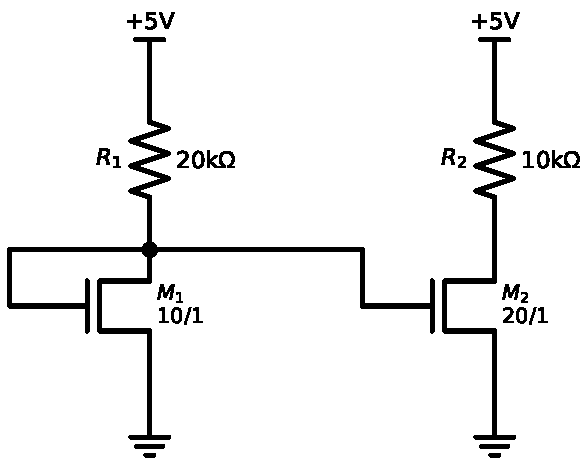
\includegraphics[width=\linewidth,height=7cm,keepaspectratio]{p01_circuit}\end{center}
\end{probbox}

\begin{probbox}{Problem 5B.2 \hfill Easy}
For the circuit below, find the DC drain currents $I_D$ of all transistors and verify their operating modes. Assume $k'_p = 100\,\mu \mathrm{A/V^2}$, $V_{tp} = -0.8$\,V (W/L next to each transistor).
\begin{center}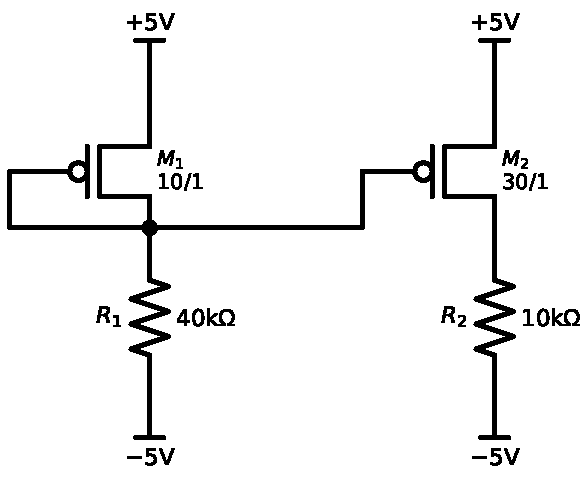
\includegraphics[width=\linewidth,height=7cm,keepaspectratio]{p02_circuit}\end{center}
\end{probbox}

\begin{probbox}{Problem 5B.3 \hfill Easy}
For the circuit below, find the DC drain currents $I_D$ of all transistors and verify their operating modes. Assume $k'_n = 200\,\mu \mathrm{A/V^2}$, $V_{tn} = 0.7$\,V (W/L next to each transistor).
\begin{center}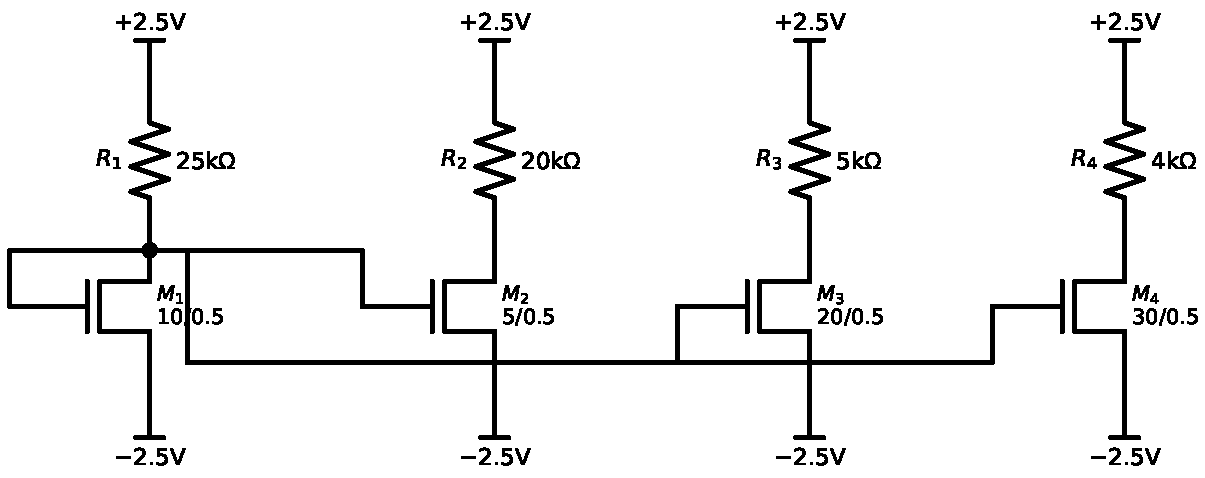
\includegraphics[width=\linewidth,height=7cm,keepaspectratio]{p03_circuit}\end{center}
\end{probbox}

\begin{probbox}{Problem 5B.4 \hfill Easy}
For the circuit below, find the DC drain currents $I_D$ of all transistors and verify their operating modes. Assume $k'_p = 100\,\mu \mathrm{A/V^2}$, $V_{tp} = -0.8$\,V (W/L next to each transistor).
\begin{center}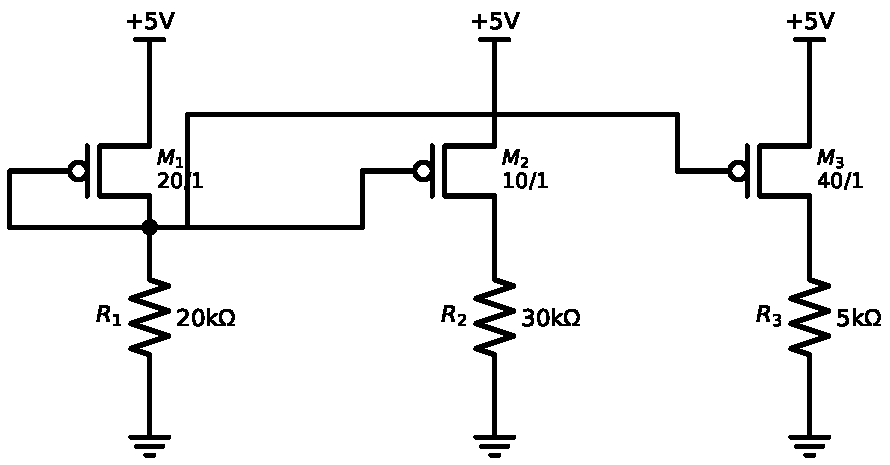
\includegraphics[width=\linewidth,height=7cm,keepaspectratio]{p04_circuit}\end{center}
\end{probbox}

\begin{probbox}{Problem 5B.5 \hfill Easy}
For the circuit below, find the DC drain currents $I_D$ of all transistors and verify their operating modes. Assume $k'_n = 200\,\mu \mathrm{A/V^2}$, $V_{tn} = 0.7$\,V (W/L next to each transistor).
\begin{center}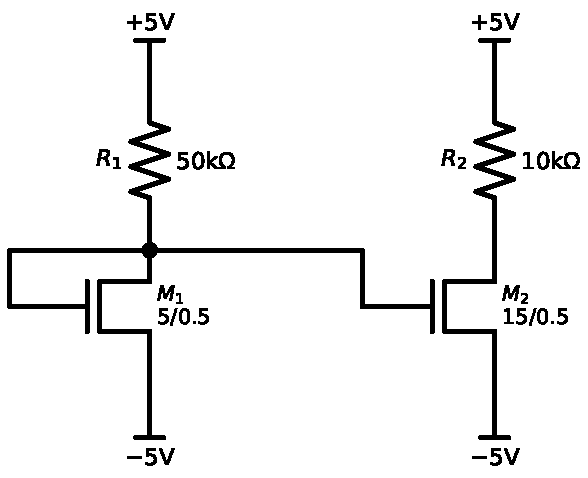
\includegraphics[width=\linewidth,height=7cm,keepaspectratio]{p05_circuit}\end{center}
\end{probbox}

\begin{probbox}{Problem 5B.6 \hfill Easy}
For the circuit below, find the DC drain currents $I_D$ of all transistors and verify their operating modes. Assume $k'_p = 100\,\mu \mathrm{A/V^2}$, $V_{tp} = -0.8$\,V (W/L next to each transistor).
\begin{center}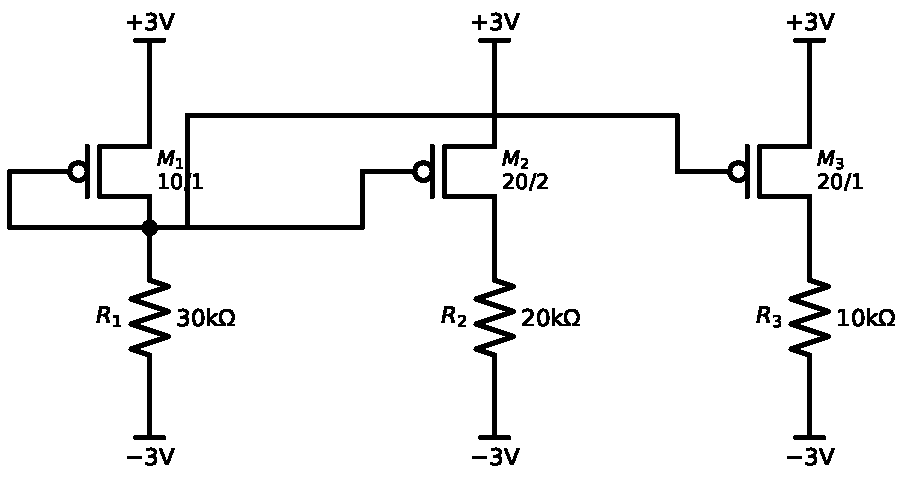
\includegraphics[width=\linewidth,height=7cm,keepaspectratio]{p06_circuit}\end{center}
\end{probbox}

\subsection*{Medium problems}
\begin{probbox}{Problem 5B.7 \hfill Medium}
For the circuit below, find the DC drain currents $I_D$ of all transistors and verify their operating modes. Assume $k'_n = 200\,\mu \mathrm{A/V^2}$, $V_{tn} = 0.7$\,V, $k'_p = 100\,\mu \mathrm{A/V^2}$, $V_{tp} = -0.8$\,V (W/L next to each transistor).
\begin{center}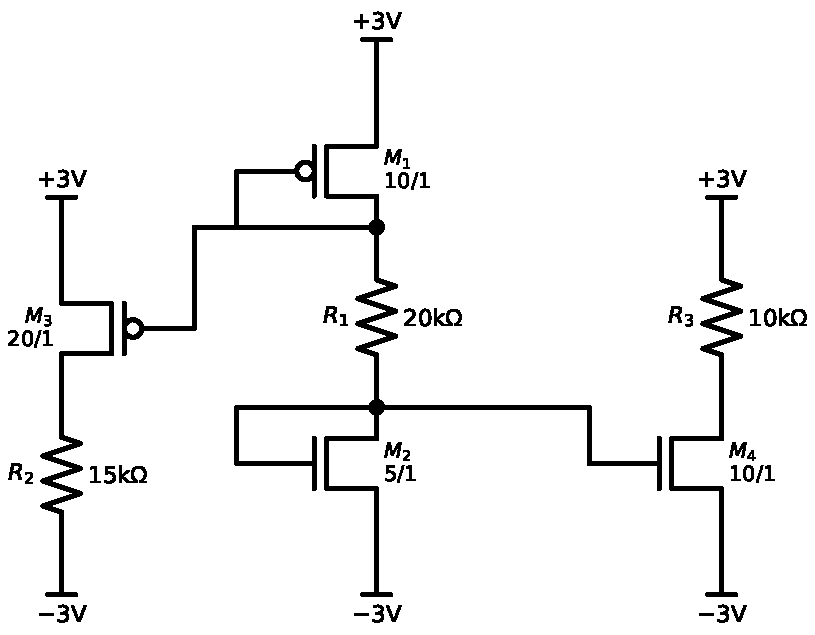
\includegraphics[width=\linewidth,height=7cm,keepaspectratio]{p07_circuit}\end{center}
\end{probbox}

\begin{probbox}{Problem 5B.8 \hfill Medium}
For the circuit below, find the DC drain currents $I_D$ of all transistors and verify their operating modes. Assume $k'_n = 200\,\mu \mathrm{A/V^2}$, $V_{tn} = 0.7$\,V, $k'_p = 100\,\mu \mathrm{A/V^2}$, $V_{tp} = -0.8$\,V (W/L next to each transistor).
\begin{center}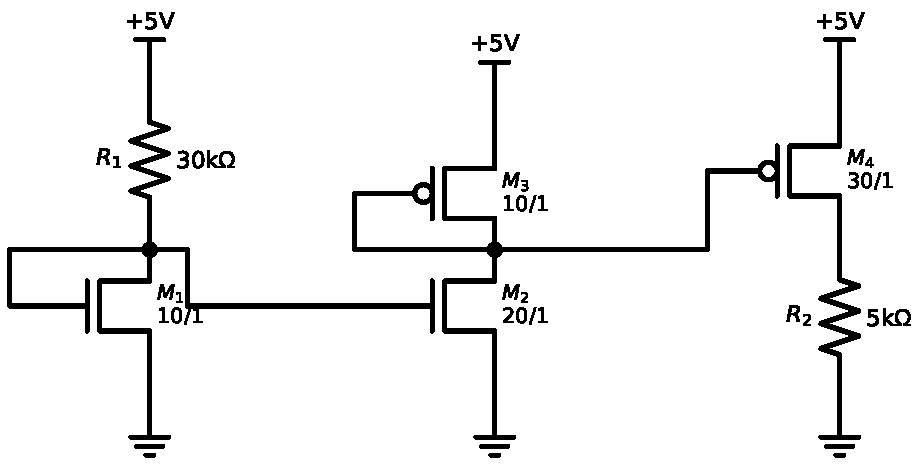
\includegraphics[width=\linewidth,height=7cm,keepaspectratio]{p08_circuit}\end{center}
\end{probbox}

\begin{probbox}{Problem 5B.9 \hfill Medium}
For the circuit below, find the DC drain currents $I_D$ of all transistors and verify their operating modes. Assume $k'_n = 200\,\mu \mathrm{A/V^2}$, $V_{tn} = 0.7$\,V (W/L next to each transistor).
\begin{center}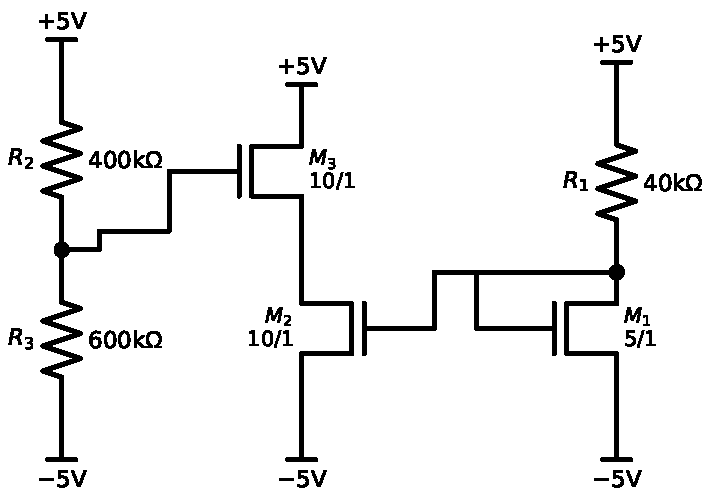
\includegraphics[width=\linewidth,height=7cm,keepaspectratio]{p09_circuit}\end{center}
\end{probbox}

\begin{probbox}{Problem 5B.10 \hfill Medium}
For the circuit below, find the DC drain currents $I_D$ of all transistors and verify their operating modes. Assume $k'_n = 200\,\mu \mathrm{A/V^2}$, $V_{tn} = 0.7$\,V, $k'_p = 100\,\mu \mathrm{A/V^2}$, $V_{tp} = -0.8$\,V (W/L next to each transistor).
\begin{center}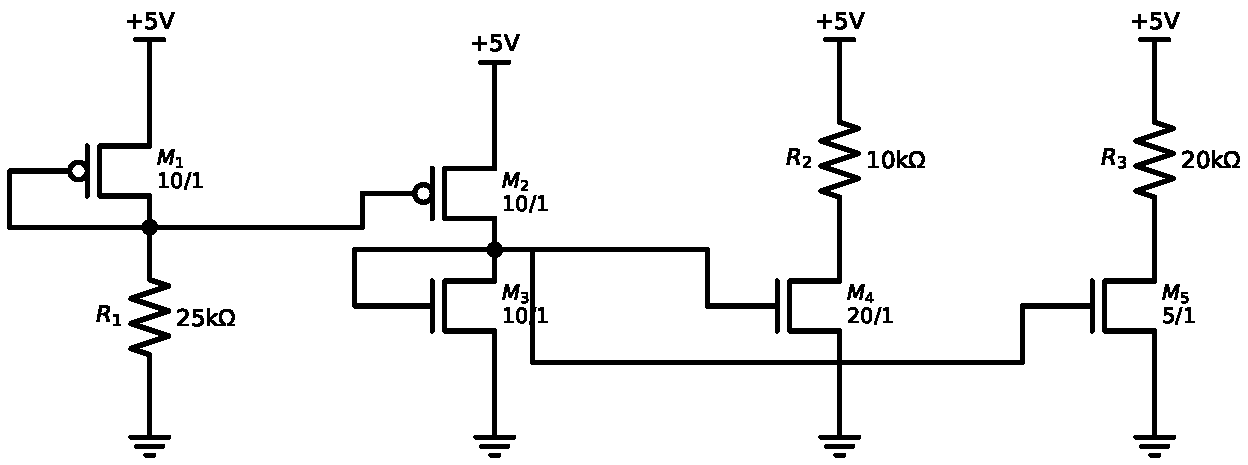
\includegraphics[width=\linewidth,height=7cm,keepaspectratio]{p10_circuit}\end{center}
\end{probbox}

\begin{probbox}{Problem 5B.11 \hfill Medium}
For the circuit below, find the DC drain currents $I_D$ of all transistors and verify their operating modes. Assume $k'_p = 100\,\mu \mathrm{A/V^2}$, $V_{tp} = -0.8$\,V (W/L next to each transistor).
\begin{center}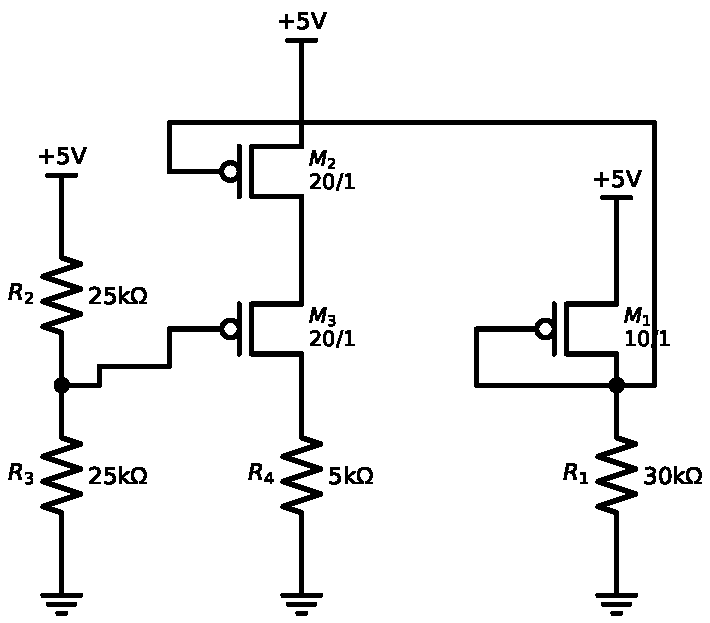
\includegraphics[width=\linewidth,height=7cm,keepaspectratio]{p11_circuit}\end{center}
\end{probbox}

\begin{probbox}{Problem 5B.12 \hfill Medium}
For the circuit below, find the DC drain currents $I_D$ of all transistors and verify their operating modes. Assume $k'_n = 200\,\mu \mathrm{A/V^2}$, $V_{tn} = 0.7$\,V (W/L next to each transistor).
\begin{center}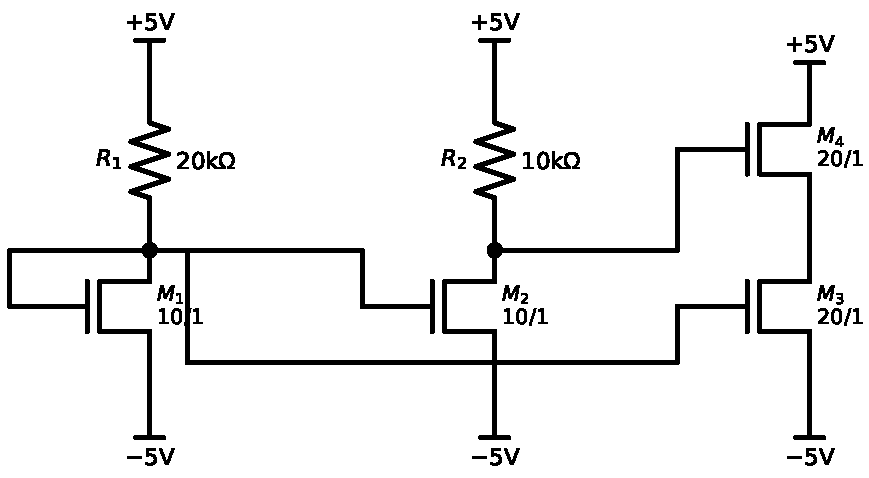
\includegraphics[width=\linewidth,height=7cm,keepaspectratio]{p12_circuit}\end{center}
\end{probbox}

\subsection*{Hard problems}
\begin{probbox}{Problem 5B.13 \hfill Hard}
For the circuit below, find the DC drain currents $I_D$ of all transistors and verify their operating modes. Assume $k'_n\frac{W}{L} = 1.1\,\mathrm{m}\mathrm{A/V^2}$, $V_{tn} = 1.4$\,V, $k'_p\frac{W}{L} = 850\,\mu \mathrm{A/V^2}$, $V_{tp} = -1.3$\,V. (This is Sample Problem 2 of the lecture.)
\begin{center}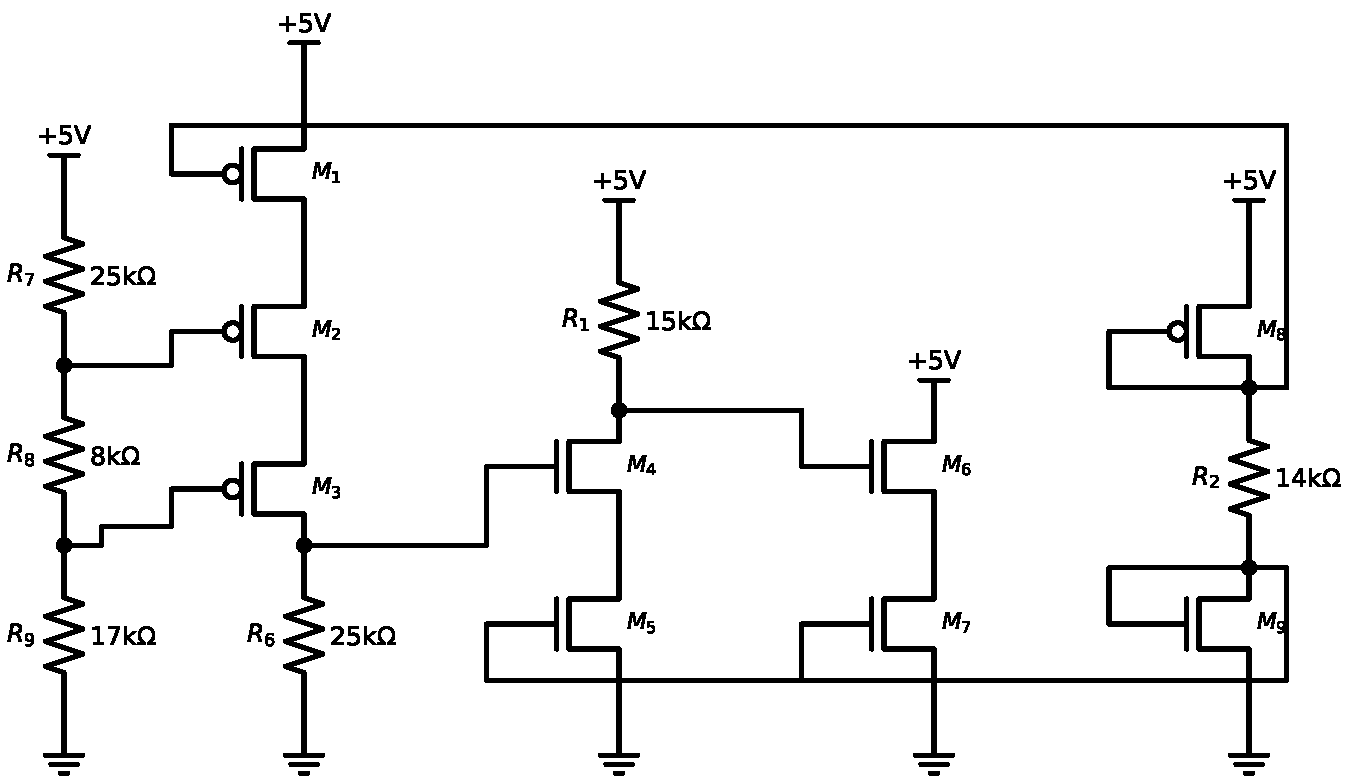
\includegraphics[width=\linewidth,height=7cm,keepaspectratio]{p13_circuit}\end{center}
\end{probbox}

\begin{probbox}{Problem 5B.14 \hfill Hard}
For the circuit below, find the DC drain currents $I_D$ of all transistors and verify their operating modes. Assume $k'_n = 200\,\mu \mathrm{A/V^2}$, $V_{tn} = 0.7$\,V, $k'_p = 100\,\mu \mathrm{A/V^2}$, $V_{tp} = -0.8$\,V (W/L next to each transistor).
\begin{center}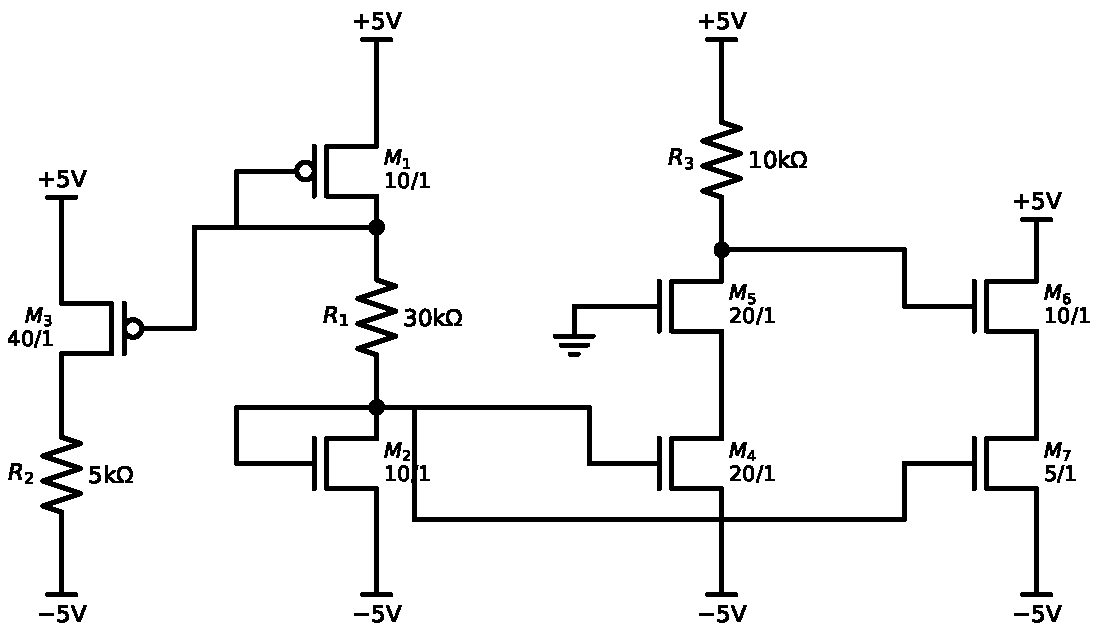
\includegraphics[width=\linewidth,height=7cm,keepaspectratio]{p14_circuit}\end{center}
\end{probbox}

\begin{probbox}{Problem 5B.15 \hfill Hard}
For the circuit below, find the DC drain currents $I_D$ of all transistors and verify their operating modes. Assume $k'_n = 200\,\mu \mathrm{A/V^2}$, $V_{tn} = 0.7$\,V, $k'_p = 100\,\mu \mathrm{A/V^2}$, $V_{tp} = -0.8$\,V (W/L next to each transistor).
\begin{center}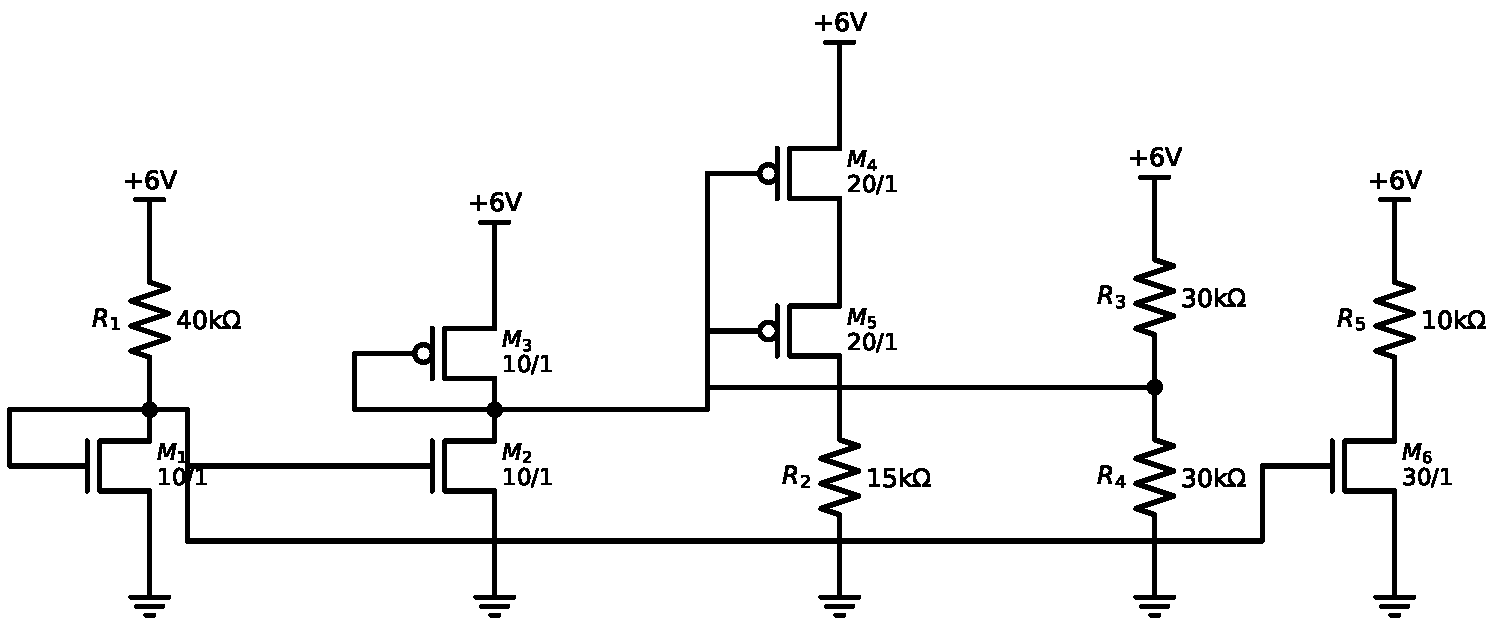
\includegraphics[width=\linewidth,height=7cm,keepaspectratio]{p15_circuit}\end{center}
\end{probbox}

\begin{probbox}{Problem 5B.16 \hfill Hard}
For the circuit below, find the DC drain currents $I_D$ of all transistors and verify their operating modes. Assume $k'_n = 200\,\mu \mathrm{A/V^2}$, $V_{tn} = 0.7$\,V, $k'_p = 100\,\mu \mathrm{A/V^2}$, $V_{tp} = -0.8$\,V (W/L next to each transistor).
\begin{center}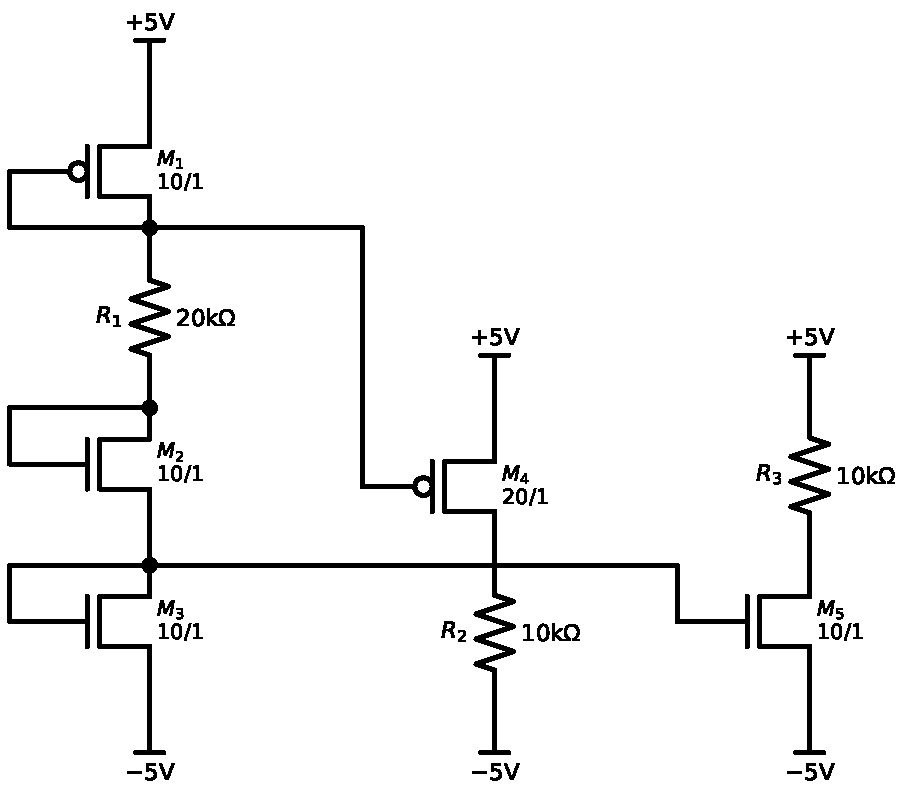
\includegraphics[width=\linewidth,height=7cm,keepaspectratio]{p16_circuit}\end{center}
\end{probbox}

\begin{probbox}{Problem 5B.17 \hfill Hard}
For the circuit below, find the DC drain currents $I_D$ of all transistors and verify their operating modes. Assume $k'_n = 200\,\mu \mathrm{A/V^2}$, $V_{tn} = 0.7$\,V, $k'_p = 100\,\mu \mathrm{A/V^2}$, $V_{tp} = -0.8$\,V (W/L next to each transistor).
\begin{center}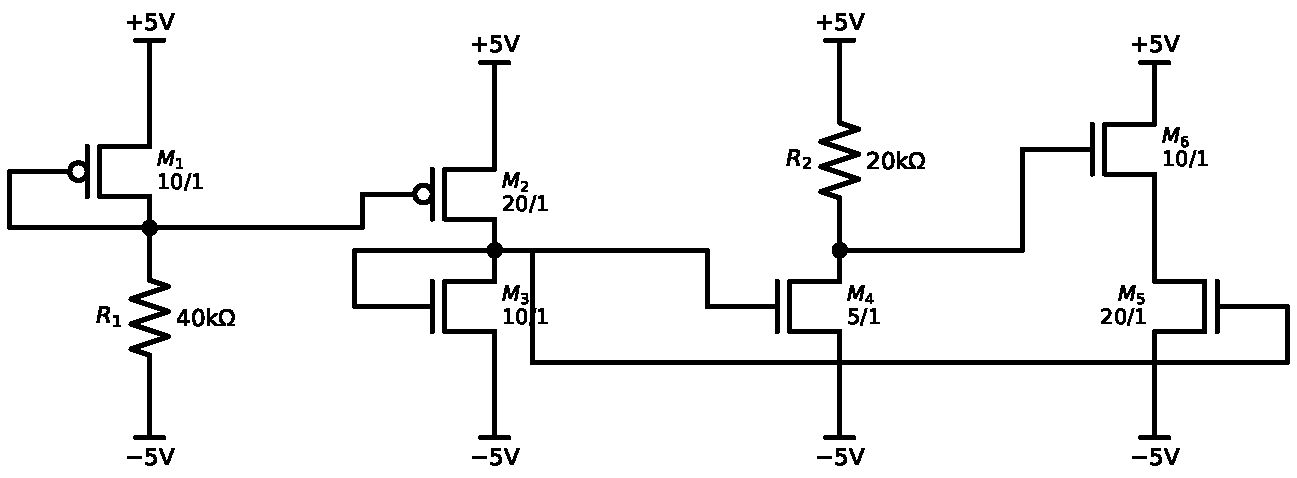
\includegraphics[width=\linewidth,height=7cm,keepaspectratio]{p17_circuit}\end{center}
\end{probbox}

\begin{probbox}{Problem 5B.18 \hfill Hard}
For the circuit below, find the DC drain currents $I_D$ of all transistors and verify their operating modes. Assume $k'_n = 200\,\mu \mathrm{A/V^2}$, $V_{tn} = 0.7$\,V, $k'_p = 100\,\mu \mathrm{A/V^2}$, $V_{tp} = -0.8$\,V (W/L next to each transistor).
\begin{center}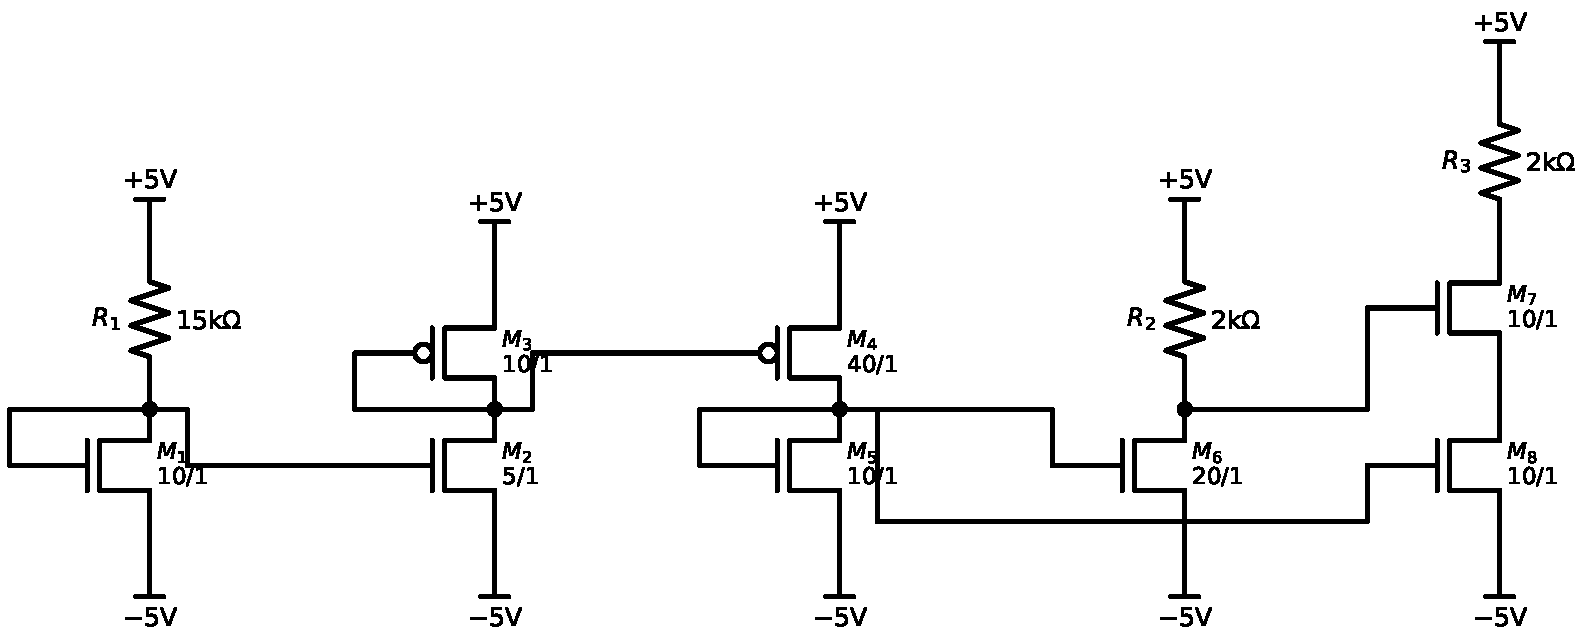
\includegraphics[width=\linewidth,height=7cm,keepaspectratio]{p18_circuit}\end{center}
\end{probbox}

\newpage
\section*{Solutions}
Every solution follows the steps of the Lecture-5 pipeline card.
\subsection*{Solution 5B.1 \hfill Easy}
\begin{center}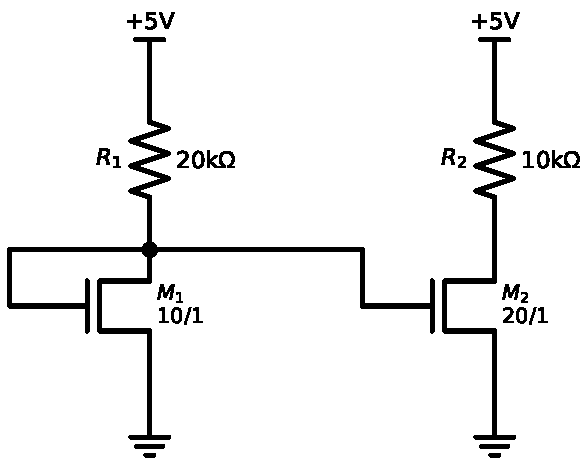
\includegraphics[width=0.9\linewidth,height=6cm,keepaspectratio]{p01_circuit}\end{center}
\solstep{1}{Assumptions}Assume every transistor is active (saturation, tool T1). No current flows into any gate, so gate voltages come from the resistor networks alone.
\solstep{2}{Walk through the circuit}\begin{enumerate}[leftmargin=*,itemsep=3pt]
\item The reference branch is one series path from $5$ to $0$: $R_{1}$, $M_{1}$. All of them carry the same current $I_D$ (gates draw none), and every diode-connected transistor is active ($V_{DS} = V_{GS} > V_{GS} - V_t$). KVL:\[5 = R_{1}I_D + V_{GS1}\]With $I_D = \frac{2\,\mathrm{m}}{2}(V_{GS1} - 0.7)^2$:\[20V_{GS1}^2 - 27V_{GS1} + 4.8 = 0 \;\Rightarrow\; V_{GS1} = 0.2106\ \text{or}\ 1.139\,\mathrm{V}\]The root $0.211$\,V is below $|V_t| = 0.7$\,V (the transistor would be off), so $V_{GS1} = 1.139$\,V. Hence $I_D = 193\,\mu \mathrm{A}$, and $V_{G1} = 1.14\,\mathrm{V}$.
\item $M_{2}$ has the same gate and source nodes as $M_{1}$, hence the same $V_{GS}$ (current mirror); the currents scale with $W/L$: $I_{D2} = I_{D1}\,\frac{\left(\frac{W}{L}\right)_{2}}{\left(\frac{W}{L}\right)_{1}} = \frac{20/1}{10/1} = 386\,\mu \mathrm{A}$.
\item $I_{D2}$ flows from $5$ through $R_{2}$: $V_{D2} = 5 - R_{2}I_{D2} = 5 - 10\,\mathrm{k}\times386\,\mu \mathrm{A} = 1.14\,\mathrm{V}$.
\end{enumerate}

\solstep{3}{Verify the operating modes}\begin{itemize}[leftmargin=*,itemsep=2pt]
\item $M_{1}$ is diode-connected: $V_{DS1} = V_{GS1} > V_{ov1}$, always active \checkmark
\item $V_{DS2} = V_{D2} - 0 = 1.139 - 0 = 1.14\,\mathrm{V}$ $\ge V_{ov2} = 0.439$\,V $\Rightarrow$ $M_{2}$ is active \checkmark
\end{itemize}
Unlike the BJT, nothing was neglected here ($I_G = 0$ exactly), so these results are exact for the square-law model: a full nodal solve of the circuit gives the same currents.
\begin{ansbox}
$I_{D1} = 193\,\mu \mathrm{A}$,\quad $I_{D2} = 386\,\mu \mathrm{A}$\\[2pt] all transistors active.
\end{ansbox}

\newpage
\subsection*{Solution 5B.2 \hfill Easy}
\begin{center}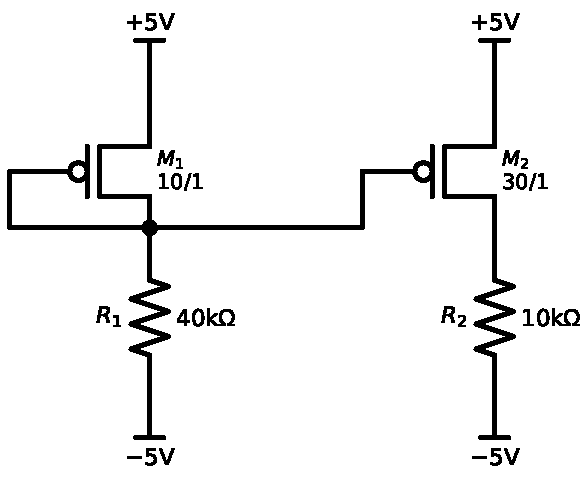
\includegraphics[width=0.9\linewidth,height=6cm,keepaspectratio]{p02_circuit}\end{center}
\solstep{1}{Assumptions}Assume every transistor is active (saturation, tool T1). No current flows into any gate, so gate voltages come from the resistor networks alone.
\solstep{2}{Walk through the circuit}\begin{enumerate}[leftmargin=*,itemsep=3pt]
\item The reference branch is one series path from $5$ to $(-5)$: $M_{1}$, $R_{1}$. All of them carry the same current $I_D$ (gates draw none), and every diode-connected transistor is active ($V_{DS} = V_{GS} > V_{GS} - V_t$). KVL:\[10 = V_{SG1} + R_{1}I_D\]With $I_D = \frac{1\,\mathrm{m}}{2}(V_{SG1} - 0.8)^2$:\[20V_{SG1}^2 - 31V_{SG1} + 2.8 = 0 \;\Rightarrow\; V_{SG1} = 0.09631\ \text{or}\ 1.454\,\mathrm{V}\]The root $0.0963$\,V is below $|V_t| = 0.8$\,V (the transistor would be off), so $V_{SG1} = 1.454$\,V. Hence $I_D = 214\,\mu \mathrm{A}$, and $V_{G1} = 3.55\,\mathrm{V}$.
\item $M_{2}$ has the same gate and source nodes as $M_{1}$, hence the same $V_{GS}$ (current mirror); the currents scale with $W/L$: $I_{D2} = I_{D1}\,\frac{\left(\frac{W}{L}\right)_{2}}{\left(\frac{W}{L}\right)_{1}} = \frac{30/1}{10/1} = 641\,\mu \mathrm{A}$.
\item $I_{D2} = 641\,\mu \mathrm{A}$ flows through $R_{2}$ to $(-5)$: $V_{D2} = (-5) + R_{2}I_{D2} = -5 + 10\,\mathrm{k}\times641\,\mu \mathrm{A} = 1.41\,\mathrm{V}$.
\end{enumerate}

\solstep{3}{Verify the operating modes}\begin{itemize}[leftmargin=*,itemsep=2pt]
\item $M_{1}$ is diode-connected: $V_{SD1} = V_{SG1} > V_{ov1}$, always active \checkmark
\item $V_{SD2} = 5 - V_{D2} = 5 - 1.41 = 3.59\,\mathrm{V}$ $\ge V_{ov2} = 0.654$\,V $\Rightarrow$ $M_{2}$ is active \checkmark
\end{itemize}
Unlike the BJT, nothing was neglected here ($I_G = 0$ exactly), so these results are exact for the square-law model: a full nodal solve of the circuit gives the same currents.
\begin{ansbox}
$I_{D1} = 214\,\mu \mathrm{A}$,\quad $I_{D2} = 641\,\mu \mathrm{A}$\\[2pt] all transistors active.
\end{ansbox}

\newpage
\subsection*{Solution 5B.3 \hfill Easy}
\begin{center}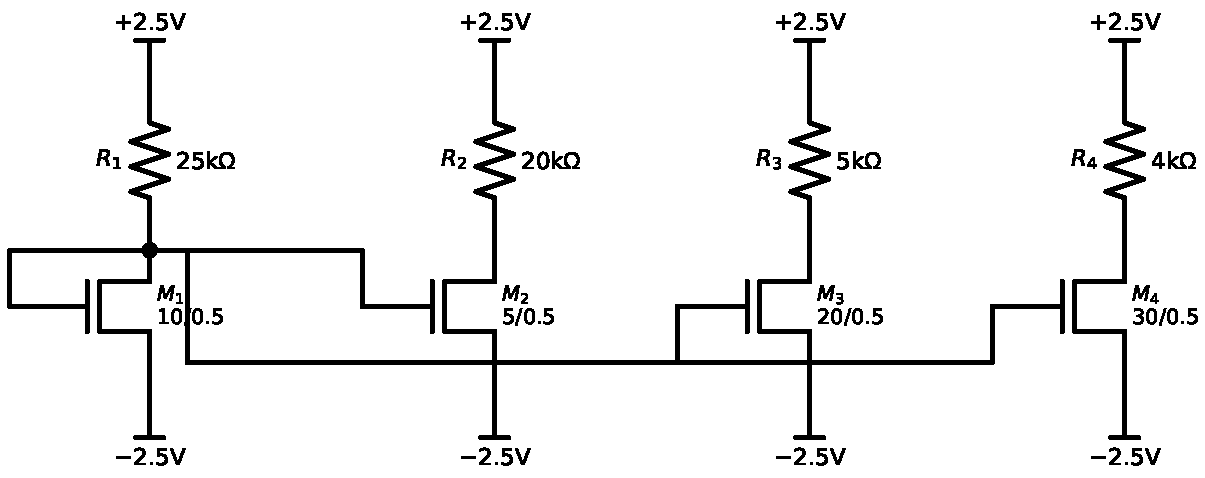
\includegraphics[width=0.9\linewidth,height=6cm,keepaspectratio]{p03_circuit}\end{center}
\solstep{1}{Assumptions}Assume every transistor is active (saturation, tool T1). No current flows into any gate, so gate voltages come from the resistor networks alone.
\solstep{2}{Walk through the circuit}\begin{enumerate}[leftmargin=*,itemsep=3pt]
\item The reference branch is one series path from $2.5$ to $(-2.5)$: $R_{1}$, $M_{1}$. All of them carry the same current $I_D$ (gates draw none), and every diode-connected transistor is active ($V_{DS} = V_{GS} > V_{GS} - V_t$). KVL:\[5 = R_{1}I_D + V_{GS1}\]With $I_D = \frac{4\,\mathrm{m}}{2}(V_{GS1} - 0.7)^2$:\[50V_{GS1}^2 - 69V_{GS1} + 19.5 = 0 \;\Rightarrow\; V_{GS1} = 0.3966\ \text{or}\ 0.9834\,\mathrm{V}\]The root $0.397$\,V is below $|V_t| = 0.7$\,V (the transistor would be off), so $V_{GS1} = 0.9834$\,V. Hence $I_D = 161\,\mu \mathrm{A}$, and $V_{G1} = -1.52\,\mathrm{V}$.
\item $M_{2}$ has the same gate and source nodes as $M_{1}$, hence the same $V_{GS}$ (current mirror); the currents scale with $W/L$: $I_{D2} = I_{D1}\,\frac{\left(\frac{W}{L}\right)_{2}}{\left(\frac{W}{L}\right)_{1}} = \frac{5/0.5}{10/0.5} = 80.3\,\mu \mathrm{A}$.
\item $M_{3}$ has the same gate and source nodes as $M_{1}$, hence the same $V_{GS}$ (current mirror); the currents scale with $W/L$: $I_{D3} = I_{D1}\,\frac{\left(\frac{W}{L}\right)_{3}}{\left(\frac{W}{L}\right)_{1}} = \frac{20/0.5}{10/0.5} = 321\,\mu \mathrm{A}$.
\item $M_{4}$ has the same gate and source nodes as $M_{1}$, hence the same $V_{GS}$ (current mirror); the currents scale with $W/L$: $I_{D4} = I_{D1}\,\frac{\left(\frac{W}{L}\right)_{4}}{\left(\frac{W}{L}\right)_{1}} = \frac{30/0.5}{10/0.5} = 482\,\mu \mathrm{A}$.
\item $I_{D2}$ flows from $2.5$ through $R_{2}$: $V_{D2} = 2.5 - R_{2}I_{D2} = 2.5 - 20\,\mathrm{k}\times80.3\,\mu \mathrm{A} = 0.893\,\mathrm{V}$.
\item $I_{D3}$ flows from $2.5$ through $R_{3}$: $V_{D3} = 2.5 - R_{3}I_{D3} = 2.5 - 5\,\mathrm{k}\times321\,\mu \mathrm{A} = 0.893\,\mathrm{V}$.
\item $I_{D4}$ flows from $2.5$ through $R_{4}$: $V_{D4} = 2.5 - R_{4}I_{D4} = 2.5 - 4\,\mathrm{k}\times482\,\mu \mathrm{A} = 0.572\,\mathrm{V}$.
\end{enumerate}

\solstep{3}{Verify the operating modes}\begin{itemize}[leftmargin=*,itemsep=2pt]
\item $M_{1}$ is diode-connected: $V_{DS1} = V_{GS1} > V_{ov1}$, always active \checkmark
\item $V_{DS2} = V_{D2} - (-2.5) = 0.8934 - (-2.5) = 3.39\,\mathrm{V}$ $\ge V_{ov2} = 0.283$\,V $\Rightarrow$ $M_{2}$ is active \checkmark
\item $V_{DS3} = V_{D3} - (-2.5) = 0.8934 - (-2.5) = 3.39\,\mathrm{V}$ $\ge V_{ov3} = 0.283$\,V $\Rightarrow$ $M_{3}$ is active \checkmark
\item $V_{DS4} = V_{D4} - (-2.5) = 0.572 - (-2.5) = 3.07\,\mathrm{V}$ $\ge V_{ov4} = 0.283$\,V $\Rightarrow$ $M_{4}$ is active \checkmark
\end{itemize}
Unlike the BJT, nothing was neglected here ($I_G = 0$ exactly), so these results are exact for the square-law model: a full nodal solve of the circuit gives the same currents.
\begin{ansbox}
$I_{D1} = 161\,\mu \mathrm{A}$,\quad $I_{D2} = 80.3\,\mu \mathrm{A}$,\quad $I_{D3} = 321\,\mu \mathrm{A}$,\quad $I_{D4} = 482\,\mu \mathrm{A}$\\[2pt] all transistors active.
\end{ansbox}

\newpage
\subsection*{Solution 5B.4 \hfill Easy}
\begin{center}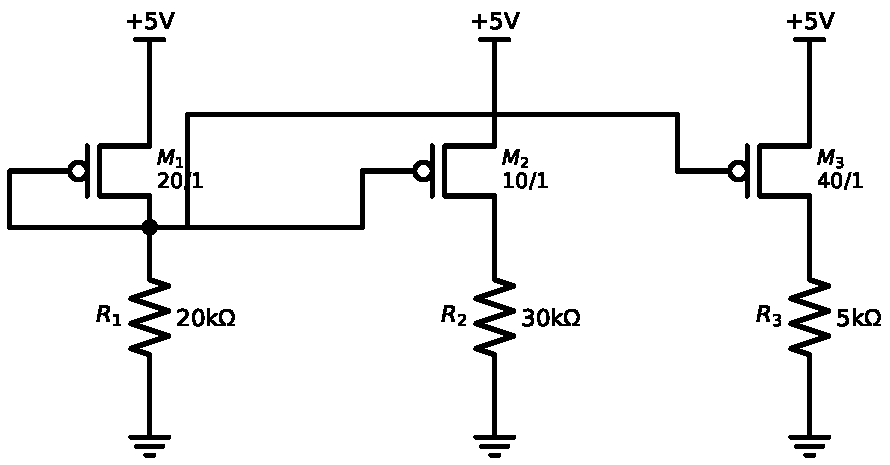
\includegraphics[width=0.9\linewidth,height=6cm,keepaspectratio]{p04_circuit}\end{center}
\solstep{1}{Assumptions}Assume every transistor is active (saturation, tool T1). No current flows into any gate, so gate voltages come from the resistor networks alone.
\solstep{2}{Walk through the circuit}\begin{enumerate}[leftmargin=*,itemsep=3pt]
\item The reference branch is one series path from $5$ to $0$: $M_{1}$, $R_{1}$. All of them carry the same current $I_D$ (gates draw none), and every diode-connected transistor is active ($V_{DS} = V_{GS} > V_{GS} - V_t$). KVL:\[5 = V_{SG1} + R_{1}I_D\]With $I_D = \frac{2\,\mathrm{m}}{2}(V_{SG1} - 0.8)^2$:\[20V_{SG1}^2 - 31V_{SG1} + 7.8 = 0 \;\Rightarrow\; V_{SG1} = 0.3161\ \text{or}\ 1.234\,\mathrm{V}\]The root $0.316$\,V is below $|V_t| = 0.8$\,V (the transistor would be off), so $V_{SG1} = 1.234$\,V. Hence $I_D = 188\,\mu \mathrm{A}$, and $V_{G1} = 3.77\,\mathrm{V}$.
\item $M_{2}$ has the same gate and source nodes as $M_{1}$, hence the same $V_{GS}$ (current mirror); the currents scale with $W/L$: $I_{D2} = I_{D1}\,\frac{\left(\frac{W}{L}\right)_{2}}{\left(\frac{W}{L}\right)_{1}} = \frac{10/1}{20/1} = 94.2\,\mu \mathrm{A}$.
\item $M_{3}$ has the same gate and source nodes as $M_{1}$, hence the same $V_{GS}$ (current mirror); the currents scale with $W/L$: $I_{D3} = I_{D1}\,\frac{\left(\frac{W}{L}\right)_{3}}{\left(\frac{W}{L}\right)_{1}} = \frac{40/1}{20/1} = 377\,\mu \mathrm{A}$.
\item $I_{D2} = 94.2\,\mu \mathrm{A}$ flows through $R_{2}$ to $0$: $V_{D2} = 0 + R_{2}I_{D2} = 0 + 30\,\mathrm{k}\times94.2\,\mu \mathrm{A} = 2.82\,\mathrm{V}$.
\item $I_{D3} = 377\,\mu \mathrm{A}$ flows through $R_{3}$ to $0$: $V_{D3} = 0 + R_{3}I_{D3} = 0 + 5\,\mathrm{k}\times377\,\mu \mathrm{A} = 1.88\,\mathrm{V}$.
\end{enumerate}

\solstep{3}{Verify the operating modes}\begin{itemize}[leftmargin=*,itemsep=2pt]
\item $M_{1}$ is diode-connected: $V_{SD1} = V_{SG1} > V_{ov1}$, always active \checkmark
\item $V_{SD2} = 5 - V_{D2} = 5 - 2.825 = 2.18\,\mathrm{V}$ $\ge V_{ov2} = 0.434$\,V $\Rightarrow$ $M_{2}$ is active \checkmark
\item $V_{SD3} = 5 - V_{D3} = 5 - 1.883 = 3.12\,\mathrm{V}$ $\ge V_{ov3} = 0.434$\,V $\Rightarrow$ $M_{3}$ is active \checkmark
\end{itemize}
Unlike the BJT, nothing was neglected here ($I_G = 0$ exactly), so these results are exact for the square-law model: a full nodal solve of the circuit gives the same currents.
\begin{ansbox}
$I_{D1} = 188\,\mu \mathrm{A}$,\quad $I_{D2} = 94.2\,\mu \mathrm{A}$,\quad $I_{D3} = 377\,\mu \mathrm{A}$\\[2pt] all transistors active.
\end{ansbox}

\newpage
\subsection*{Solution 5B.5 \hfill Easy}
\begin{center}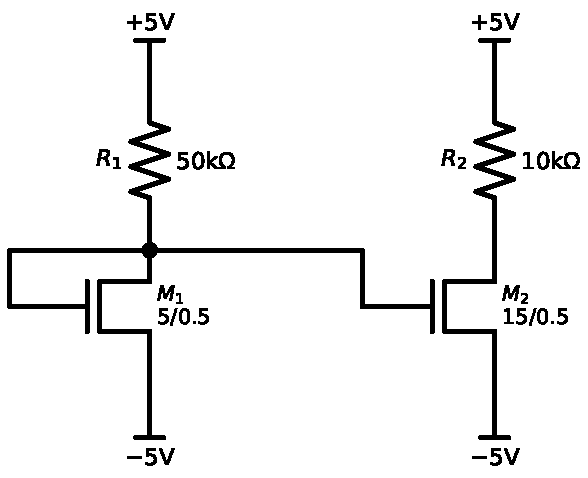
\includegraphics[width=0.9\linewidth,height=6cm,keepaspectratio]{p05_circuit}\end{center}
\solstep{1}{Assumptions}Assume every transistor is active (saturation, tool T1). No current flows into any gate, so gate voltages come from the resistor networks alone.
\solstep{2}{Walk through the circuit}\begin{enumerate}[leftmargin=*,itemsep=3pt]
\item The reference branch is one series path from $5$ to $(-5)$: $R_{1}$, $M_{1}$. All of them carry the same current $I_D$ (gates draw none), and every diode-connected transistor is active ($V_{DS} = V_{GS} > V_{GS} - V_t$). KVL:\[10 = R_{1}I_D + V_{GS1}\]With $I_D = \frac{2\,\mathrm{m}}{2}(V_{GS1} - 0.7)^2$:\[50V_{GS1}^2 - 69V_{GS1} + 14.5 = 0 \;\Rightarrow\; V_{GS1} = 0.2586\ \text{or}\ 1.121\,\mathrm{V}\]The root $0.259$\,V is below $|V_t| = 0.7$\,V (the transistor would be off), so $V_{GS1} = 1.121$\,V. Hence $I_D = 178\,\mu \mathrm{A}$, and $V_{G1} = -3.88\,\mathrm{V}$.
\item $M_{2}$ has the same gate and source nodes as $M_{1}$, hence the same $V_{GS}$ (current mirror); the currents scale with $W/L$: $I_{D2} = I_{D1}\,\frac{\left(\frac{W}{L}\right)_{2}}{\left(\frac{W}{L}\right)_{1}} = \frac{15/0.5}{5/0.5} = 533\,\mu \mathrm{A}$.
\item $I_{D2}$ flows from $5$ through $R_{2}$: $V_{D2} = 5 - R_{2}I_{D2} = 5 - 10\,\mathrm{k}\times533\,\mu \mathrm{A} = -0.327\,\mathrm{V}$.
\end{enumerate}

\solstep{3}{Verify the operating modes}\begin{itemize}[leftmargin=*,itemsep=2pt]
\item $M_{1}$ is diode-connected: $V_{DS1} = V_{GS1} > V_{ov1}$, always active \checkmark
\item $V_{DS2} = V_{D2} - (-5) = -0.3272 - (-5) = 4.67\,\mathrm{V}$ $\ge V_{ov2} = 0.421$\,V $\Rightarrow$ $M_{2}$ is active \checkmark
\end{itemize}
Unlike the BJT, nothing was neglected here ($I_G = 0$ exactly), so these results are exact for the square-law model: a full nodal solve of the circuit gives the same currents.
\begin{ansbox}
$I_{D1} = 178\,\mu \mathrm{A}$,\quad $I_{D2} = 533\,\mu \mathrm{A}$\\[2pt] all transistors active.
\end{ansbox}

\newpage
\subsection*{Solution 5B.6 \hfill Easy}
\begin{center}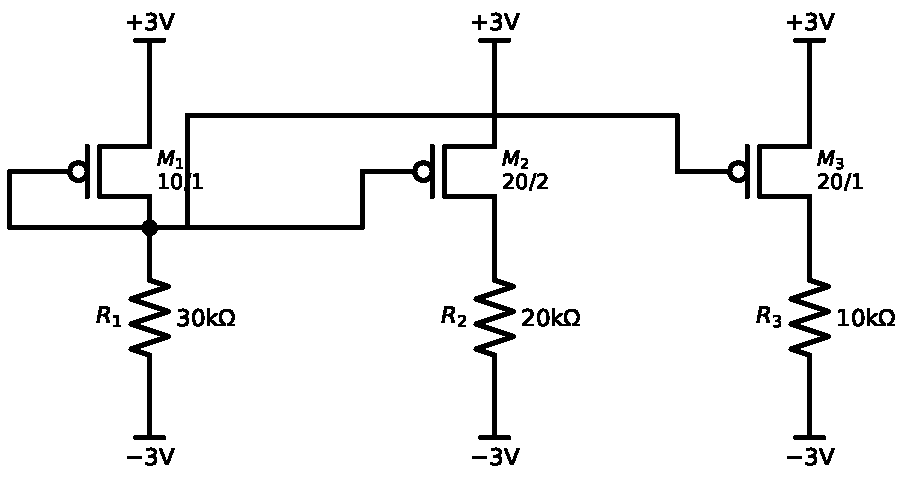
\includegraphics[width=0.9\linewidth,height=6cm,keepaspectratio]{p06_circuit}\end{center}
\solstep{1}{Assumptions}Assume every transistor is active (saturation, tool T1). No current flows into any gate, so gate voltages come from the resistor networks alone.
\solstep{2}{Walk through the circuit}\begin{enumerate}[leftmargin=*,itemsep=3pt]
\item The reference branch is one series path from $3$ to $(-3)$: $M_{1}$, $R_{1}$. All of them carry the same current $I_D$ (gates draw none), and every diode-connected transistor is active ($V_{DS} = V_{GS} > V_{GS} - V_t$). KVL:\[6 = V_{SG1} + R_{1}I_D\]With $I_D = \frac{1\,\mathrm{m}}{2}(V_{SG1} - 0.8)^2$:\[15V_{SG1}^2 - 23V_{SG1} + 3.6 = 0 \;\Rightarrow\; V_{SG1} = 0.1769\ \text{or}\ 1.356\,\mathrm{V}\]The root $0.177$\,V is below $|V_t| = 0.8$\,V (the transistor would be off), so $V_{SG1} = 1.356$\,V. Hence $I_D = 155\,\mu \mathrm{A}$, and $V_{G1} = 1.64\,\mathrm{V}$.
\item $M_{2}$ has the same gate and source nodes as $M_{1}$, hence the same $V_{GS}$ (current mirror): $I_{D2} = I_{D1} = 155\,\mu \mathrm{A}$.
\item $M_{3}$ has the same gate and source nodes as $M_{1}$, hence the same $V_{GS}$ (current mirror); the currents scale with $W/L$: $I_{D3} = I_{D1}\,\frac{\left(\frac{W}{L}\right)_{3}}{\left(\frac{W}{L}\right)_{1}} = \frac{20/1}{10/1} = 310\,\mu \mathrm{A}$.
\item $I_{D2} = 155\,\mu \mathrm{A}$ flows through $R_{2}$ to $(-3)$: $V_{D2} = (-3) + R_{2}I_{D2} = -3 + 20\,\mathrm{k}\times155\,\mu \mathrm{A} = 0.0957\,\mathrm{V}$.
\item $I_{D3} = 310\,\mu \mathrm{A}$ flows through $R_{3}$ to $(-3)$: $V_{D3} = (-3) + R_{3}I_{D3} = -3 + 10\,\mathrm{k}\times310\,\mu \mathrm{A} = 0.0957\,\mathrm{V}$.
\end{enumerate}

\solstep{3}{Verify the operating modes}\begin{itemize}[leftmargin=*,itemsep=2pt]
\item $M_{1}$ is diode-connected: $V_{SD1} = V_{SG1} > V_{ov1}$, always active \checkmark
\item $V_{SD2} = 3 - V_{D2} = 3 - 0.09574 = 2.9\,\mathrm{V}$ $\ge V_{ov2} = 0.556$\,V $\Rightarrow$ $M_{2}$ is active \checkmark
\item $V_{SD3} = 3 - V_{D3} = 3 - 0.09574 = 2.9\,\mathrm{V}$ $\ge V_{ov3} = 0.556$\,V $\Rightarrow$ $M_{3}$ is active \checkmark
\end{itemize}
Unlike the BJT, nothing was neglected here ($I_G = 0$ exactly), so these results are exact for the square-law model: a full nodal solve of the circuit gives the same currents.
\begin{ansbox}
$I_{D1} = 155\,\mu \mathrm{A}$,\quad $I_{D2} = 155\,\mu \mathrm{A}$,\quad $I_{D3} = 310\,\mu \mathrm{A}$\\[2pt] all transistors active.
\end{ansbox}

\newpage
\subsection*{Solution 5B.7 \hfill Medium}
\begin{center}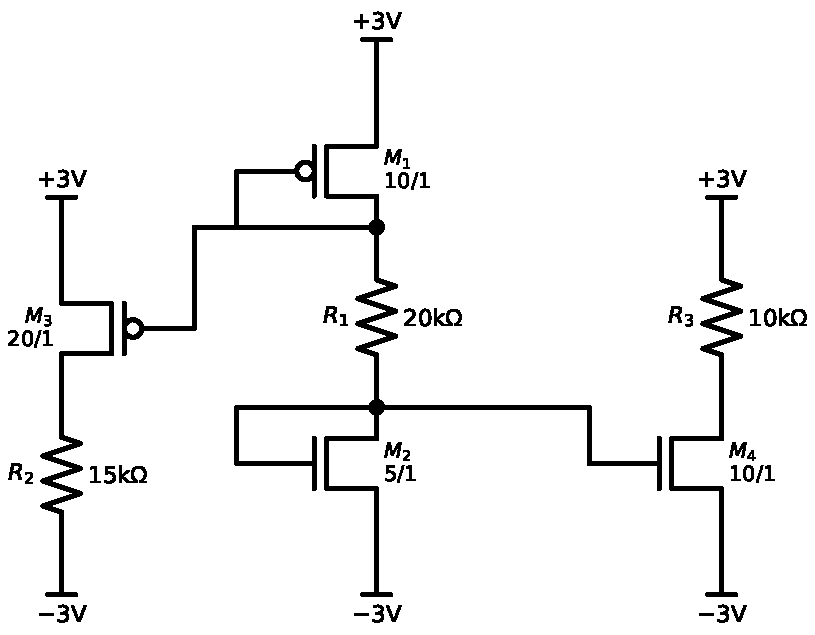
\includegraphics[width=0.9\linewidth,height=6cm,keepaspectratio]{p07_circuit}\end{center}
\solstep{1}{Assumptions}Assume every transistor is active (saturation, tool T1). No current flows into any gate, so gate voltages come from the resistor networks alone.
\solstep{2}{Walk through the circuit}\begin{enumerate}[leftmargin=*,itemsep=3pt]
\item The reference branch is one series path from $3$ to $(-3)$: $M_{1}$, $R_{1}$, $M_{2}$. All of them carry the same current $I_D$ (gates draw none), and every diode-connected transistor is active ($V_{DS} = V_{GS} > V_{GS} - V_t$). KVL:\[6 = V_{SG1} + R_{1}I_D + V_{GS2}\]Equal currents, $\frac{k_i}{2}V_{ov,i}^2$ the same for all, give $V_{ov2} = V_{ov1}\sqrt{k_{1}/k_{2}} = 1\,V_{ov1}$. With $I_D = \frac{1\,\mathrm{m}}{2}(V_{SG1} - 0.8)^2$ everything is a function of $V_{SG1}$:\[10V_{SG1}^2 - 14V_{SG1} + 0.3 = 0 \;\Rightarrow\; V_{SG1} = 0.02177\ \text{or}\ 1.378\,\mathrm{V}\]The root $0.0218$\,V is below $|V_t| = 0.8$\,V (the transistor would be off), so $V_{SG1} = 1.378$\,V. Hence $I_D = 167\,\mu \mathrm{A}$, $V_{GS2} = 1.278$\,V, and $V_{G3} = 1.62\,\mathrm{V}$, $V_{G2} = -1.72\,\mathrm{V}$.
\item $M_{3}$ has the same gate and source nodes as $M_{1}$, hence the same $V_{GS}$ (current mirror); the currents scale with $W/L$: $I_{D3} = I_{D1}\,\frac{\left(\frac{W}{L}\right)_{3}}{\left(\frac{W}{L}\right)_{1}} = \frac{20/1}{10/1} = 334\,\mu \mathrm{A}$.
\item $M_{4}$ has the same gate and source nodes as $M_{2}$, hence the same $V_{GS}$ (current mirror); the currents scale with $W/L$: $I_{D4} = I_{D2}\,\frac{\left(\frac{W}{L}\right)_{4}}{\left(\frac{W}{L}\right)_{2}} = \frac{10/1}{5/1} = 334\,\mu \mathrm{A}$.
\item $I_{D3} = 334\,\mu \mathrm{A}$ flows through $R_{2}$ to $(-3)$: $V_{D3} = (-3) + R_{2}I_{D3} = -3 + 15\,\mathrm{k}\times334\,\mu \mathrm{A} = 2.02\,\mathrm{V}$.
\item $I_{D4}$ flows from $3$ through $R_{3}$: $V_{D4} = 3 - R_{3}I_{D4} = 3 - 10\,\mathrm{k}\times334\,\mu \mathrm{A} = -0.344\,\mathrm{V}$.
\end{enumerate}

\solstep{3}{Verify the operating modes}\begin{itemize}[leftmargin=*,itemsep=2pt]
\item $V_{SD3} = 3 - V_{D3} = 3 - 2.015 = 0.985\,\mathrm{V}$ $\ge V_{ov3} = 0.578$\,V $\Rightarrow$ $M_{3}$ is active \checkmark
\item $M_{1}$ is diode-connected: $V_{SD1} = V_{SG1} > V_{ov1}$, always active \checkmark
\item $M_{2}$ is diode-connected: $V_{DS2} = V_{GS2} > V_{ov2}$, always active \checkmark
\item $V_{DS4} = V_{D4} - (-3) = -0.3435 - (-3) = 2.66\,\mathrm{V}$ $\ge V_{ov4} = 0.578$\,V $\Rightarrow$ $M_{4}$ is active \checkmark
\end{itemize}
Unlike the BJT, nothing was neglected here ($I_G = 0$ exactly), so these results are exact for the square-law model: a full nodal solve of the circuit gives the same currents.
\begin{ansbox}
$I_{D3} = 334\,\mu \mathrm{A}$,\quad $I_{D1} = 167\,\mu \mathrm{A}$,\quad $I_{D2} = 167\,\mu \mathrm{A}$,\quad $I_{D4} = 334\,\mu \mathrm{A}$\\[2pt] all transistors active.
\end{ansbox}

\newpage
\subsection*{Solution 5B.8 \hfill Medium}
\begin{center}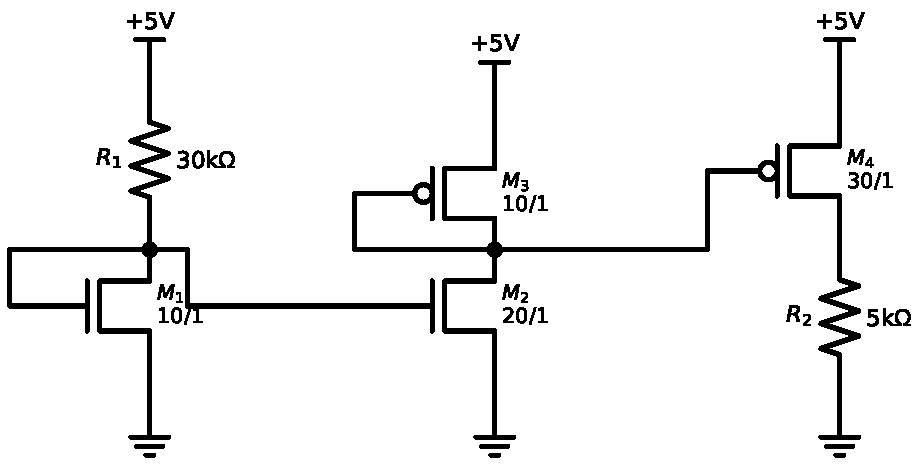
\includegraphics[width=0.9\linewidth,height=6cm,keepaspectratio]{p08_circuit}\end{center}
\solstep{1}{Assumptions}Assume every transistor is active (saturation, tool T1). No current flows into any gate, so gate voltages come from the resistor networks alone.
\solstep{2}{Walk through the circuit}\begin{enumerate}[leftmargin=*,itemsep=3pt]
\item The reference branch is one series path from $5$ to $0$: $R_{1}$, $M_{1}$. All of them carry the same current $I_D$ (gates draw none), and every diode-connected transistor is active ($V_{DS} = V_{GS} > V_{GS} - V_t$). KVL:\[5 = R_{1}I_D + V_{GS1}\]With $I_D = \frac{2\,\mathrm{m}}{2}(V_{GS1} - 0.7)^2$:\[30V_{GS1}^2 - 41V_{GS1} + 9.7 = 0 \;\Rightarrow\; V_{GS1} = 0.3044\ \text{or}\ 1.062\,\mathrm{V}\]The root $0.304$\,V is below $|V_t| = 0.7$\,V (the transistor would be off), so $V_{GS1} = 1.062$\,V. Hence $I_D = 131\,\mu \mathrm{A}$, and $V_{G1} = 1.06\,\mathrm{V}$.
\item $M_{2}$ has the same gate and source nodes as $M_{1}$, hence the same $V_{GS}$ (current mirror); the currents scale with $W/L$: $I_{D2} = I_{D1}\,\frac{\left(\frac{W}{L}\right)_{2}}{\left(\frac{W}{L}\right)_{1}} = \frac{20/1}{10/1} = 263\,\mu \mathrm{A}$.
\item $M_{3}$ is in series with $M_{2}$ (nothing else draws current at $V_{G3}$): $I_{D3} = I_{D2} = 263\,\mu \mathrm{A}$.
\item $M_{4}$ has the same gate and source nodes as $M_{3}$, hence the same $V_{GS}$ (current mirror); the currents scale with $W/L$: $I_{D4} = I_{D3}\,\frac{\left(\frac{W}{L}\right)_{4}}{\left(\frac{W}{L}\right)_{3}} = \frac{30/1}{10/1} = 788\,\mu \mathrm{A}$.
\item $M_{3}$ carries $I_{D3} = 263\,\mu \mathrm{A}$, so $V_{ov3} = \sqrt{2I_{D3}/k_{3}} = 0.7246$\,V and $V_{SG3} = 1.525$\,V: $V_{G3} = 5 - V_{SG3} = 3.48\,\mathrm{V}$ (diode-connected: this is also its drain voltage).
\item $I_{D4} = 788\,\mu \mathrm{A}$ flows through $R_{2}$ to $0$: $V_{D4} = 0 + R_{2}I_{D4} = 0 + 5\,\mathrm{k}\times788\,\mu \mathrm{A} = 3.94\,\mathrm{V}$.
\end{enumerate}

\solstep{3}{Verify the operating modes}\begin{itemize}[leftmargin=*,itemsep=2pt]
\item $M_{1}$ is diode-connected: $V_{DS1} = V_{GS1} > V_{ov1}$, always active \checkmark
\item $M_{3}$ is diode-connected: $V_{SD3} = V_{SG3} > V_{ov3}$, always active \checkmark
\item $V_{DS2} = V_{G3} - 0 = 3.475 - 0 = 3.48\,\mathrm{V}$ $\ge V_{ov2} = 0.362$\,V $\Rightarrow$ $M_{2}$ is active \checkmark
\item $V_{SD4} = 5 - V_{D4} = 5 - 3.938 = 1.06\,\mathrm{V}$ $\ge V_{ov4} = 0.725$\,V $\Rightarrow$ $M_{4}$ is active \checkmark
\end{itemize}
Unlike the BJT, nothing was neglected here ($I_G = 0$ exactly), so these results are exact for the square-law model: a full nodal solve of the circuit gives the same currents.
\begin{ansbox}
$I_{D1} = 131\,\mu \mathrm{A}$,\quad $I_{D3} = 263\,\mu \mathrm{A}$,\quad $I_{D2} = 263\,\mu \mathrm{A}$,\quad $I_{D4} = 788\,\mu \mathrm{A}$\\[2pt] all transistors active.
\end{ansbox}

\newpage
\subsection*{Solution 5B.9 \hfill Medium}
\begin{center}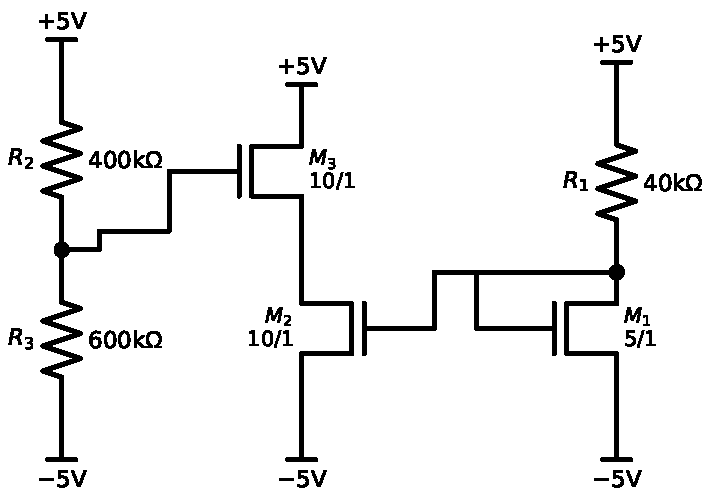
\includegraphics[width=0.9\linewidth,height=6cm,keepaspectratio]{p09_circuit}\end{center}
\solstep{1}{Assumptions}Assume every transistor is active (saturation, tool T1). No current flows into any gate, so gate voltages come from the resistor networks alone.
\solstep{2}{Walk through the circuit}\begin{enumerate}[leftmargin=*,itemsep=3pt]
\item No current flows into a gate ($I_G = 0$), so $V_{G3}$ is set by the divider $R_{2}$--$R_{3}$:\[V_{G3} = -5 + (5 - (-5))\frac{600\,\mathrm{k}}{400\,\mathrm{k} + 600\,\mathrm{k}} = 1\,\mathrm{V}\]
\item The reference branch is one series path from $5$ to $(-5)$: $R_{1}$, $M_{1}$. All of them carry the same current $I_D$ (gates draw none), and every diode-connected transistor is active ($V_{DS} = V_{GS} > V_{GS} - V_t$). KVL:\[10 = R_{1}I_D + V_{GS1}\]With $I_D = \frac{1\,\mathrm{m}}{2}(V_{GS1} - 0.7)^2$:\[20V_{GS1}^2 - 27V_{GS1} - 0.2 = 0 \;\Rightarrow\; V_{GS1} = -0.007367\ \text{or}\ 1.357\,\mathrm{V}\]The root $-0.00737$\,V is below $|V_t| = 0.7$\,V (the transistor would be off), so $V_{GS1} = 1.357$\,V. Hence $I_D = 216\,\mu \mathrm{A}$, and $V_{G2} = -3.64\,\mathrm{V}$.
\item $M_{2}$ has the same gate and source nodes as $M_{1}$, hence the same $V_{GS}$ (current mirror); the currents scale with $W/L$: $I_{D2} = I_{D1}\,\frac{\left(\frac{W}{L}\right)_{2}}{\left(\frac{W}{L}\right)_{1}} = \frac{10/1}{5/1} = 432\,\mu \mathrm{A}$.
\item $M_{3}$ is in series with $M_{2}$ (nothing else draws current at $V_{S3}$): $I_{D3} = I_{D2} = 432\,\mu \mathrm{A}$.
\item $M_{3}$ carries $I_{D3} = 432\,\mu \mathrm{A}$, so $V_{ov3} = \sqrt{2I_{D3}/k_{3}} = 0.6574$\,V and $V_{GS3} = 0.7 + 0.6574 = 1.357$\,V: $V_{S3} = V_{G3} - V_{GS3} = -0.357\,\mathrm{V}$.
\end{enumerate}

\solstep{3}{Verify the operating modes}\begin{itemize}[leftmargin=*,itemsep=2pt]
\item $V_{DS3} = 5 - V_{S3} = 5 - (-0.3574) = 5.36\,\mathrm{V}$ $\ge V_{ov3} = 0.657$\,V $\Rightarrow$ $M_{3}$ is active \checkmark
\item $V_{DS2} = V_{S3} - (-5) = -0.3574 - (-5) = 4.64\,\mathrm{V}$ $\ge V_{ov2} = 0.657$\,V $\Rightarrow$ $M_{2}$ is active \checkmark
\item $M_{1}$ is diode-connected: $V_{DS1} = V_{GS1} > V_{ov1}$, always active \checkmark
\end{itemize}
Unlike the BJT, nothing was neglected here ($I_G = 0$ exactly), so these results are exact for the square-law model: a full nodal solve of the circuit gives the same currents.
\begin{ansbox}
$I_{D3} = 432\,\mu \mathrm{A}$,\quad $I_{D2} = 432\,\mu \mathrm{A}$,\quad $I_{D1} = 216\,\mu \mathrm{A}$\\[2pt] all transistors active.
\end{ansbox}

\newpage
\subsection*{Solution 5B.10 \hfill Medium}
\begin{center}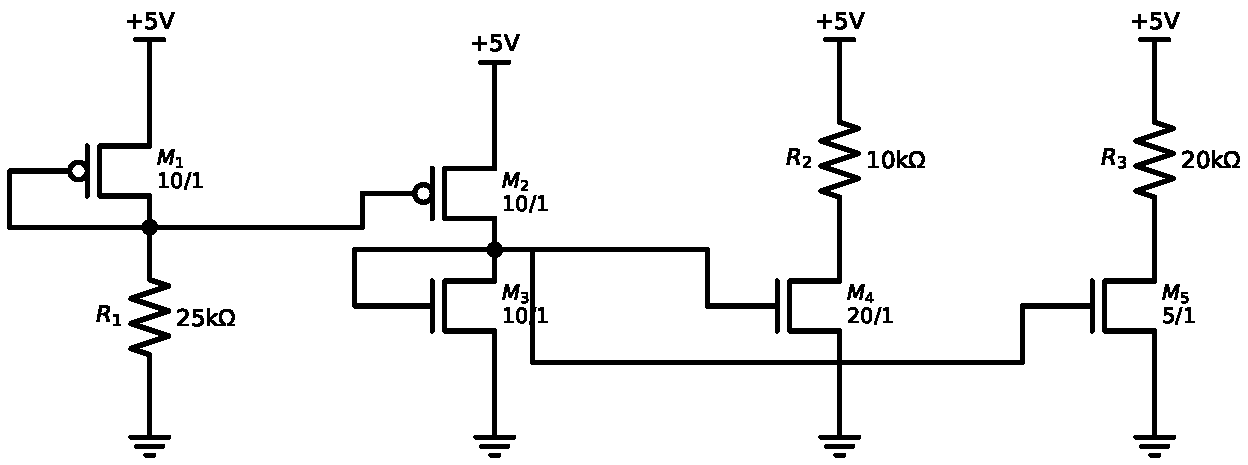
\includegraphics[width=0.9\linewidth,height=6cm,keepaspectratio]{p10_circuit}\end{center}
\solstep{1}{Assumptions}Assume every transistor is active (saturation, tool T1). No current flows into any gate, so gate voltages come from the resistor networks alone.
\solstep{2}{Walk through the circuit}\begin{enumerate}[leftmargin=*,itemsep=3pt]
\item The reference branch is one series path from $5$ to $0$: $M_{1}$, $R_{1}$. All of them carry the same current $I_D$ (gates draw none), and every diode-connected transistor is active ($V_{DS} = V_{GS} > V_{GS} - V_t$). KVL:\[5 = V_{SG1} + R_{1}I_D\]With $I_D = \frac{1\,\mathrm{m}}{2}(V_{SG1} - 0.8)^2$:\[12.5V_{SG1}^2 - 19V_{SG1} + 3 = 0 \;\Rightarrow\; V_{SG1} = 0.179\ \text{or}\ 1.341\,\mathrm{V}\]The root $0.179$\,V is below $|V_t| = 0.8$\,V (the transistor would be off), so $V_{SG1} = 1.341$\,V. Hence $I_D = 146\,\mu \mathrm{A}$, and $V_{G1} = 3.66\,\mathrm{V}$.
\item $M_{2}$ has the same gate and source nodes as $M_{1}$, hence the same $V_{GS}$ (current mirror): $I_{D2} = I_{D1} = 146\,\mu \mathrm{A}$.
\item $M_{3}$ is in series with $M_{2}$ (nothing else draws current at $V_{D2}$): $I_{D3} = I_{D2} = 146\,\mu \mathrm{A}$.
\item $M_{4}$ has the same gate and source nodes as $M_{3}$, hence the same $V_{GS}$ (current mirror); the currents scale with $W/L$: $I_{D4} = I_{D3}\,\frac{\left(\frac{W}{L}\right)_{4}}{\left(\frac{W}{L}\right)_{3}} = \frac{20/1}{10/1} = 293\,\mu \mathrm{A}$.
\item $M_{5}$ has the same gate and source nodes as $M_{3}$, hence the same $V_{GS}$ (current mirror); the currents scale with $W/L$: $I_{D5} = I_{D3}\,\frac{\left(\frac{W}{L}\right)_{5}}{\left(\frac{W}{L}\right)_{3}} = \frac{5/1}{10/1} = 73.2\,\mu \mathrm{A}$.
\item $M_{3}$ carries $I_{D3} = 146\,\mu \mathrm{A}$, so $V_{ov3} = \sqrt{2I_{D3}/k_{3}} = 0.3826$\,V and $V_{GS3} = 1.083$\,V: $V_{D2} = 0 + V_{GS3} = 1.08\,\mathrm{V}$ (diode-connected: this is also its drain voltage).
\item $I_{D4}$ flows from $5$ through $R_{2}$: $V_{D4} = 5 - R_{2}I_{D4} = 5 - 10\,\mathrm{k}\times293\,\mu \mathrm{A} = 2.07\,\mathrm{V}$.
\item $I_{D5}$ flows from $5$ through $R_{3}$: $V_{D5} = 5 - R_{3}I_{D5} = 5 - 20\,\mathrm{k}\times73.2\,\mu \mathrm{A} = 3.54\,\mathrm{V}$.
\end{enumerate}

\solstep{3}{Verify the operating modes}\begin{itemize}[leftmargin=*,itemsep=2pt]
\item $M_{1}$ is diode-connected: $V_{SD1} = V_{SG1} > V_{ov1}$, always active \checkmark
\item $V_{SD2} = 5 - V_{D2} = 5 - 1.083 = 3.92\,\mathrm{V}$ $\ge V_{ov2} = 0.541$\,V $\Rightarrow$ $M_{2}$ is active \checkmark
\item $M_{3}$ is diode-connected: $V_{DS3} = V_{GS3} > V_{ov3}$, always active \checkmark
\item $V_{DS4} = V_{D4} - 0 = 2.073 - 0 = 2.07\,\mathrm{V}$ $\ge V_{ov4} = 0.383$\,V $\Rightarrow$ $M_{4}$ is active \checkmark
\item $V_{DS5} = V_{D5} - 0 = 3.536 - 0 = 3.54\,\mathrm{V}$ $\ge V_{ov5} = 0.383$\,V $\Rightarrow$ $M_{5}$ is active \checkmark
\end{itemize}
Unlike the BJT, nothing was neglected here ($I_G = 0$ exactly), so these results are exact for the square-law model: a full nodal solve of the circuit gives the same currents.
\begin{ansbox}
$I_{D1} = 146\,\mu \mathrm{A}$,\quad $I_{D2} = 146\,\mu \mathrm{A}$,\quad $I_{D3} = 146\,\mu \mathrm{A}$,\quad $I_{D4} = 293\,\mu \mathrm{A}$,\quad $I_{D5} = 73.2\,\mu \mathrm{A}$\\[2pt] all transistors active.
\end{ansbox}

\newpage
\subsection*{Solution 5B.11 \hfill Medium}
\begin{center}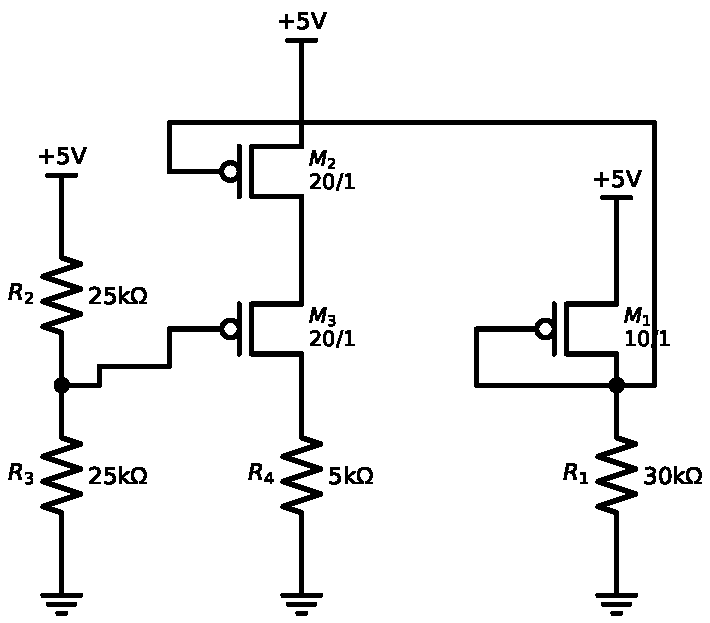
\includegraphics[width=0.9\linewidth,height=6cm,keepaspectratio]{p11_circuit}\end{center}
\solstep{1}{Assumptions}Assume every transistor is active (saturation, tool T1). No current flows into any gate, so gate voltages come from the resistor networks alone.
\solstep{2}{Walk through the circuit}\begin{enumerate}[leftmargin=*,itemsep=3pt]
\item No current flows into a gate ($I_G = 0$), so $V_{G3}$ is set by the divider $R_{2}$--$R_{3}$:\[V_{G3} = 0 + (5 - 0)\frac{25\,\mathrm{k}}{25\,\mathrm{k} + 25\,\mathrm{k}} = 2.5\,\mathrm{V}\]
\item The reference branch is one series path from $5$ to $0$: $M_{1}$, $R_{1}$. All of them carry the same current $I_D$ (gates draw none), and every diode-connected transistor is active ($V_{DS} = V_{GS} > V_{GS} - V_t$). KVL:\[5 = V_{SG1} + R_{1}I_D\]With $I_D = \frac{1\,\mathrm{m}}{2}(V_{SG1} - 0.8)^2$:\[15V_{SG1}^2 - 23V_{SG1} + 4.6 = 0 \;\Rightarrow\; V_{SG1} = 0.2365\ \text{or}\ 1.297\,\mathrm{V}\]The root $0.236$\,V is below $|V_t| = 0.8$\,V (the transistor would be off), so $V_{SG1} = 1.297$\,V. Hence $I_D = 123\,\mu \mathrm{A}$, and $V_{G2} = 3.7\,\mathrm{V}$.
\item $M_{2}$ has the same gate and source nodes as $M_{1}$, hence the same $V_{GS}$ (current mirror); the currents scale with $W/L$: $I_{D2} = I_{D1}\,\frac{\left(\frac{W}{L}\right)_{2}}{\left(\frac{W}{L}\right)_{1}} = \frac{20/1}{10/1} = 247\,\mu \mathrm{A}$.
\item $M_{3}$ is in series with $M_{2}$ (nothing else draws current at $V_{D2}$): $I_{D3} = I_{D2} = 247\,\mu \mathrm{A}$.
\item $I_{D3} = 247\,\mu \mathrm{A}$ flows through $R_{4}$ to $0$: $V_{D3} = 0 + R_{4}I_{D3} = 0 + 5\,\mathrm{k}\times247\,\mu \mathrm{A} = 1.23\,\mathrm{V}$.
\item $M_{3}$ carries $I_{D3} = 247\,\mu \mathrm{A}$, so $V_{ov3} = \sqrt{2I_{D3}/k_{3}} = 0.4969$\,V and $V_{SG3} = 0.8 + 0.4969 = 1.297$\,V: $V_{D2} = V_{G3} + V_{SG3} = 3.8\,\mathrm{V}$.
\end{enumerate}

\solstep{3}{Verify the operating modes}\begin{itemize}[leftmargin=*,itemsep=2pt]
\item $V_{SD2} = 5 - V_{D2} = 5 - 3.797 = 1.2\,\mathrm{V}$ $\ge V_{ov2} = 0.497$\,V $\Rightarrow$ $M_{2}$ is active \checkmark
\item $V_{SD3} = V_{D2} - V_{D3} = 3.797 - 1.234 = 2.56\,\mathrm{V}$ $\ge V_{ov3} = 0.497$\,V $\Rightarrow$ $M_{3}$ is active \checkmark
\item $M_{1}$ is diode-connected: $V_{SD1} = V_{SG1} > V_{ov1}$, always active \checkmark
\end{itemize}
Unlike the BJT, nothing was neglected here ($I_G = 0$ exactly), so these results are exact for the square-law model: a full nodal solve of the circuit gives the same currents.
\begin{ansbox}
$I_{D2} = 247\,\mu \mathrm{A}$,\quad $I_{D3} = 247\,\mu \mathrm{A}$,\quad $I_{D1} = 123\,\mu \mathrm{A}$\\[2pt] all transistors active.
\end{ansbox}

\newpage
\subsection*{Solution 5B.12 \hfill Medium}
\begin{center}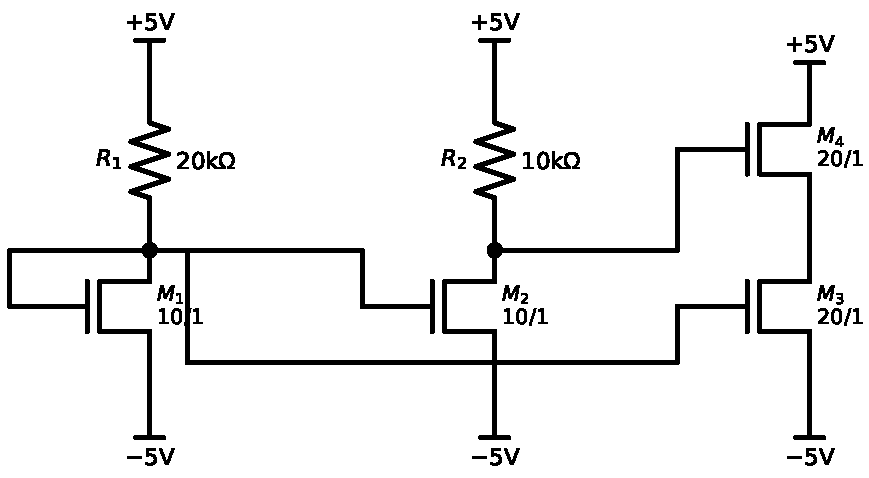
\includegraphics[width=0.9\linewidth,height=6cm,keepaspectratio]{p12_circuit}\end{center}
\solstep{1}{Assumptions}Assume every transistor is active (saturation, tool T1). No current flows into any gate, so gate voltages come from the resistor networks alone.
\solstep{2}{Walk through the circuit}\begin{enumerate}[leftmargin=*,itemsep=3pt]
\item The reference branch is one series path from $5$ to $(-5)$: $R_{1}$, $M_{1}$. All of them carry the same current $I_D$ (gates draw none), and every diode-connected transistor is active ($V_{DS} = V_{GS} > V_{GS} - V_t$). KVL:\[10 = R_{1}I_D + V_{GS1}\]With $I_D = \frac{2\,\mathrm{m}}{2}(V_{GS1} - 0.7)^2$:\[20V_{GS1}^2 - 27V_{GS1} - 0.2 = 0 \;\Rightarrow\; V_{GS1} = -0.007367\ \text{or}\ 1.357\,\mathrm{V}\]The root $-0.00737$\,V is below $|V_t| = 0.7$\,V (the transistor would be off), so $V_{GS1} = 1.357$\,V. Hence $I_D = 432\,\mu \mathrm{A}$, and $V_{G1} = -3.64\,\mathrm{V}$.
\item $M_{2}$ has the same gate and source nodes as $M_{1}$, hence the same $V_{GS}$ (current mirror): $I_{D2} = I_{D1} = 432\,\mu \mathrm{A}$.
\item $M_{3}$ has the same gate and source nodes as $M_{1}$, hence the same $V_{GS}$ (current mirror); the currents scale with $W/L$: $I_{D3} = I_{D1}\,\frac{\left(\frac{W}{L}\right)_{3}}{\left(\frac{W}{L}\right)_{1}} = \frac{20/1}{10/1} = 864\,\mu \mathrm{A}$.
\item $I_{D2}$ flows from $5$ through $R_{2}$: $V_{D2} = 5 - R_{2}I_{D2} = 5 - 10\,\mathrm{k}\times432\,\mu \mathrm{A} = 0.679\,\mathrm{V}$.
\item $M_{4}$ is in series with $M_{3}$ (nothing else draws current at $V_{S4}$): $I_{D4} = I_{D3} = 864\,\mu \mathrm{A}$.
\item $M_{4}$ carries $I_{D4} = 864\,\mu \mathrm{A}$, so $V_{ov4} = \sqrt{2I_{D4}/k_{4}} = 0.6574$\,V and $V_{GS4} = 0.7 + 0.6574 = 1.357$\,V: $V_{S4} = V_{D2} - V_{GS4} = -0.679\,\mathrm{V}$.
\end{enumerate}

\solstep{3}{Verify the operating modes}\begin{itemize}[leftmargin=*,itemsep=2pt]
\item $M_{1}$ is diode-connected: $V_{DS1} = V_{GS1} > V_{ov1}$, always active \checkmark
\item $V_{DS2} = V_{D2} - (-5) = 0.6787 - (-5) = 5.68\,\mathrm{V}$ $\ge V_{ov2} = 0.657$\,V $\Rightarrow$ $M_{2}$ is active \checkmark
\item $V_{DS4} = 5 - V_{S4} = 5 - (-0.6787) = 5.68\,\mathrm{V}$ $\ge V_{ov4} = 0.657$\,V $\Rightarrow$ $M_{4}$ is active \checkmark
\item $V_{DS3} = V_{S4} - (-5) = -0.6787 - (-5) = 4.32\,\mathrm{V}$ $\ge V_{ov3} = 0.657$\,V $\Rightarrow$ $M_{3}$ is active \checkmark
\end{itemize}
Unlike the BJT, nothing was neglected here ($I_G = 0$ exactly), so these results are exact for the square-law model: a full nodal solve of the circuit gives the same currents.
\begin{ansbox}
$I_{D1} = 432\,\mu \mathrm{A}$,\quad $I_{D2} = 432\,\mu \mathrm{A}$,\quad $I_{D4} = 864\,\mu \mathrm{A}$,\quad $I_{D3} = 864\,\mu \mathrm{A}$\\[2pt] all transistors active.
\end{ansbox}

\newpage
\subsection*{Solution 5B.13 \hfill Hard}
\begin{center}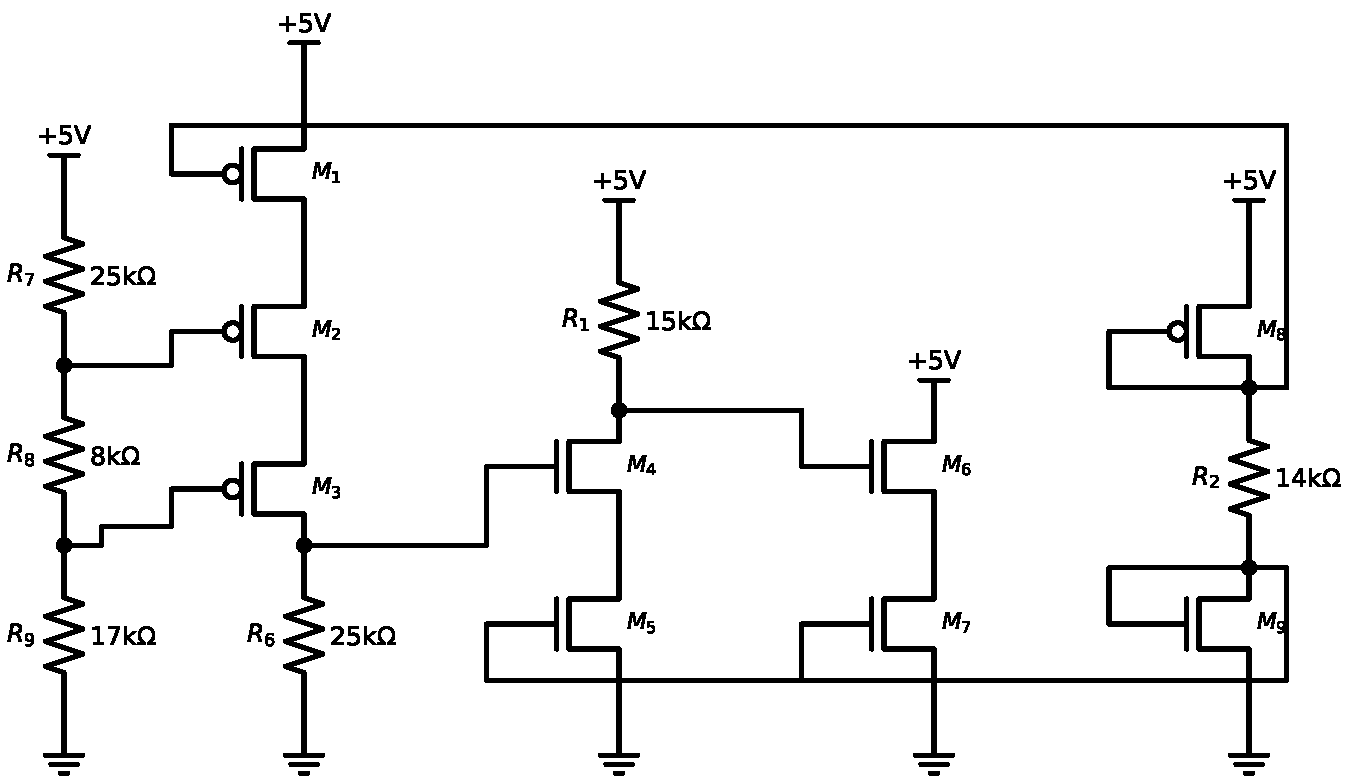
\includegraphics[width=0.9\linewidth,height=6cm,keepaspectratio]{p13_circuit}\end{center}
\solstep{1}{Assumptions}Assume every transistor is active (saturation, tool T1). No current flows into any gate, so gate voltages come from the resistor networks alone.
\solstep{2}{Walk through the circuit}\begin{enumerate}[leftmargin=*,itemsep=3pt]
\item No current flows into a gate ($I_G = 0$), so the string $R_{7}$--$R_{8}$--$R_{9}$ carries one current: $I = \frac{5 - 0}{25\,\mathrm{k} + 8\,\mathrm{k} + 17\,\mathrm{k}} = 100\,\mu \mathrm{A}$. Hence $V_{G2} = 5 - (25\,\mathrm{k})\times100\,\mu \mathrm{A} = 2.5\,\mathrm{V}$, $V_{G3} = 5 - (25\,\mathrm{k} + 8\,\mathrm{k})\times100\,\mu \mathrm{A} = 1.7\,\mathrm{V}$.
\item The reference branch is one series path from $5$ to $0$: $M_{8}$, $R_{2}$, $M_{9}$. All of them carry the same current $I_D$ (gates draw none), and every diode-connected transistor is active ($V_{DS} = V_{GS} > V_{GS} - V_t$). KVL:\[5 = V_{SG8} + R_{2}I_D + V_{GS9}\]Equal currents, $\frac{k_i}{2}V_{ov,i}^2$ the same for all, give $V_{ov9} = V_{ov8}\sqrt{k_{8}/k_{9}} = 0.879\,V_{ov8}$. With $I_D = \frac{850\,\mu }{2}(V_{SG8} - 1.3)^2$ everything is a function of $V_{SG8}$:\[5.95V_{SG8}^2 - 13.59V_{SG8} + 5.313 = 0 \;\Rightarrow\; V_{SG8} = 0.5006\ \text{or}\ 1.784\,\mathrm{V}\]The root $0.501$\,V is below $|V_t| = 1.3$\,V (the transistor would be off), so $V_{SG8} = 1.784$\,V. Hence $I_D = 99.4\,\mu \mathrm{A}$, $V_{GS9} = 1.825$\,V, and $V_{G1} = 3.22\,\mathrm{V}$, $V_{G5} = 1.83\,\mathrm{V}$.
\item $M_{1}$ has the same gate and source nodes as $M_{8}$, hence the same $V_{GS}$ (current mirror): $I_{D1} = I_{D8} = 99.4\,\mu \mathrm{A}$.
\item $M_{5}$ has the same gate and source nodes as $M_{9}$, hence the same $V_{GS}$ (current mirror): $I_{D5} = I_{D9} = 99.4\,\mu \mathrm{A}$.
\item $M_{7}$ has the same gate and source nodes as $M_{9}$, hence the same $V_{GS}$ (current mirror): $I_{D7} = I_{D9} = 99.4\,\mu \mathrm{A}$.
\item $M_{2}$ is in series with $M_{1}$ (nothing else draws current at $V_{D1}$): $I_{D2} = I_{D1} = 99.4\,\mu \mathrm{A}$.
\item $M_{2}$ carries $I_{D2} = 99.4\,\mu \mathrm{A}$, so $V_{ov2} = \sqrt{2I_{D2}/k_{2}} = 0.4836$\,V and $V_{SG2} = 1.3 + 0.4836 = 1.784$\,V: $V_{D1} = V_{G2} + V_{SG2} = 4.28\,\mathrm{V}$.
\item $M_{3}$ is in series with $M_{2}$ (nothing else draws current at $V_{D2}$): $I_{D3} = I_{D2} = 99.4\,\mu \mathrm{A}$.
\item $I_{D3} = 99.4\,\mu \mathrm{A}$ flows through $R_{6}$ to $0$: $V_{D3} = 0 + R_{6}I_{D3} = 0 + 25\,\mathrm{k}\times99.4\,\mu \mathrm{A} = 2.48\,\mathrm{V}$.
\item $M_{3}$ carries $I_{D3} = 99.4\,\mu \mathrm{A}$, so $V_{ov3} = \sqrt{2I_{D3}/k_{3}} = 0.4836$\,V and $V_{SG3} = 1.3 + 0.4836 = 1.784$\,V: $V_{D2} = V_{G3} + V_{SG3} = 3.48\,\mathrm{V}$.
\item $M_{4}$ is in series with $M_{5}$ (nothing else draws current at $V_{S4}$): $I_{D4} = I_{D5} = 99.4\,\mu \mathrm{A}$.
\item $I_{D4}$ flows from $5$ through $R_{1}$: $V_{D4} = 5 - R_{1}I_{D4} = 5 - 15\,\mathrm{k}\times99.4\,\mu \mathrm{A} = 3.51\,\mathrm{V}$.
\item $M_{4}$ carries $I_{D4} = 99.4\,\mu \mathrm{A}$, so $V_{ov4} = \sqrt{2I_{D4}/k_{4}} = 0.4251$\,V and $V_{GS4} = 1.4 + 0.4251 = 1.825$\,V: $V_{S4} = V_{D3} - V_{GS4} = 0.659\,\mathrm{V}$.
\item $M_{6}$ is in series with $M_{7}$ (nothing else draws current at $V_{S6}$): $I_{D6} = I_{D7} = 99.4\,\mu \mathrm{A}$.
\item $M_{6}$ carries $I_{D6} = 99.4\,\mu \mathrm{A}$, so $V_{ov6} = \sqrt{2I_{D6}/k_{6}} = 0.4251$\,V and $V_{GS6} = 1.4 + 0.4251 = 1.825$\,V: $V_{S6} = V_{D4} - V_{GS6} = 1.68\,\mathrm{V}$.
\end{enumerate}

\solstep{3}{Verify the operating modes}\begin{itemize}[leftmargin=*,itemsep=2pt]
\item $V_{SD1} = 5 - V_{D1} = 5 - 4.284 = 0.716\,\mathrm{V}$ $\ge V_{ov1} = 0.484$\,V $\Rightarrow$ $M_{1}$ is active \checkmark
\item $V_{SD2} = V_{D1} - V_{D2} = 4.284 - 3.484 = 0.8\,\mathrm{V}$ $\ge V_{ov2} = 0.484$\,V $\Rightarrow$ $M_{2}$ is active \checkmark
\item $V_{SD3} = V_{D2} - V_{D3} = 3.484 - 2.485 = 0.999\,\mathrm{V}$ $\ge V_{ov3} = 0.484$\,V $\Rightarrow$ $M_{3}$ is active \checkmark
\item $V_{DS4} = V_{D4} - V_{S4} = 3.509 - 0.6595 = 2.85\,\mathrm{V}$ $\ge V_{ov4} = 0.425$\,V $\Rightarrow$ $M_{4}$ is active \checkmark
\item $V_{DS5} = V_{S4} - 0 = 0.6595 - 0 = 0.659\,\mathrm{V}$ $\ge V_{ov5} = 0.425$\,V $\Rightarrow$ $M_{5}$ is active \checkmark
\item $V_{DS6} = 5 - V_{S6} = 5 - 1.684 = 3.32\,\mathrm{V}$ $\ge V_{ov6} = 0.425$\,V $\Rightarrow$ $M_{6}$ is active \checkmark
\item $V_{DS7} = V_{S6} - 0 = 1.684 - 0 = 1.68\,\mathrm{V}$ $\ge V_{ov7} = 0.425$\,V $\Rightarrow$ $M_{7}$ is active \checkmark
\item $M_{8}$ is diode-connected: $V_{SD8} = V_{SG8} > V_{ov8}$, always active \checkmark
\item $M_{9}$ is diode-connected: $V_{DS9} = V_{GS9} > V_{ov9}$, always active \checkmark
\end{itemize}
Unlike the BJT, nothing was neglected here ($I_G = 0$ exactly), so these results are exact for the square-law model: a full nodal solve of the circuit gives the same currents.
\begin{ansbox}
$I_{D1} = 99.4\,\mu \mathrm{A}$,\quad $I_{D2} = 99.4\,\mu \mathrm{A}$,\quad $I_{D3} = 99.4\,\mu \mathrm{A}$,\quad $I_{D4} = 99.4\,\mu \mathrm{A}$,\quad $I_{D5} = 99.4\,\mu \mathrm{A}$,\quad $I_{D6} = 99.4\,\mu \mathrm{A}$,\quad $I_{D7} = 99.4\,\mu \mathrm{A}$,\quad $I_{D8} = 99.4\,\mu \mathrm{A}$,\quad $I_{D9} = 99.4\,\mu \mathrm{A}$\\[2pt] all transistors active.
\end{ansbox}

\newpage
\subsection*{Solution 5B.14 \hfill Hard}
\begin{center}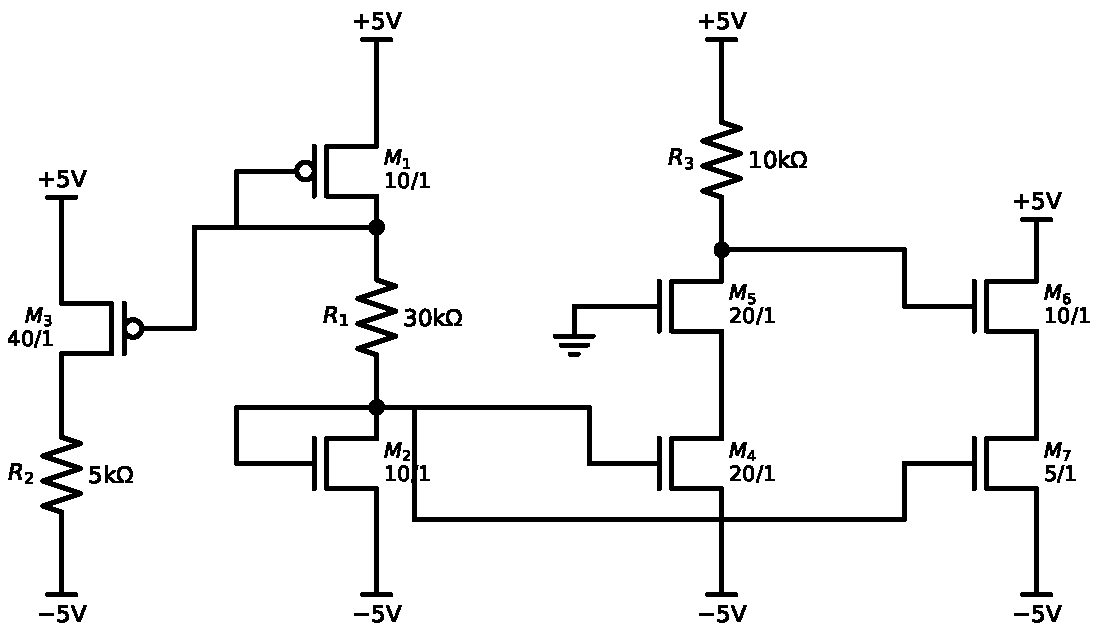
\includegraphics[width=0.9\linewidth,height=6cm,keepaspectratio]{p14_circuit}\end{center}
\solstep{1}{Assumptions}Assume every transistor is active (saturation, tool T1). No current flows into any gate, so gate voltages come from the resistor networks alone.
\solstep{2}{Walk through the circuit}\begin{enumerate}[leftmargin=*,itemsep=3pt]
\item The reference branch is one series path from $5$ to $(-5)$: $M_{1}$, $R_{1}$, $M_{2}$. All of them carry the same current $I_D$ (gates draw none), and every diode-connected transistor is active ($V_{DS} = V_{GS} > V_{GS} - V_t$). KVL:\[10 = V_{SG1} + R_{1}I_D + V_{GS2}\]Equal currents, $\frac{k_i}{2}V_{ov,i}^2$ the same for all, give $V_{ov2} = V_{ov1}\sqrt{k_{1}/k_{2}} = 0.7071\,V_{ov1}$. With $I_D = \frac{1\,\mathrm{m}}{2}(V_{SG1} - 0.8)^2$ everything is a function of $V_{SG1}$:\[15V_{SG1}^2 - 22.29V_{SG1} - 0.2657 = 0 \;\Rightarrow\; V_{SG1} = -0.01182\ \text{or}\ 1.498\,\mathrm{V}\]The root $-0.0118$\,V is below $|V_t| = 0.8$\,V (the transistor would be off), so $V_{SG1} = 1.498$\,V. Hence $I_D = 244\,\mu \mathrm{A}$, $V_{GS2} = 1.194$\,V, and $V_{G3} = 3.5\,\mathrm{V}$, $V_{G2} = -3.81\,\mathrm{V}$.
\item $M_{3}$ has the same gate and source nodes as $M_{1}$, hence the same $V_{GS}$ (current mirror); the currents scale with $W/L$: $I_{D3} = I_{D1}\,\frac{\left(\frac{W}{L}\right)_{3}}{\left(\frac{W}{L}\right)_{1}} = \frac{40/1}{10/1} = 974\,\mu \mathrm{A}$.
\item $M_{4}$ has the same gate and source nodes as $M_{2}$, hence the same $V_{GS}$ (current mirror); the currents scale with $W/L$: $I_{D4} = I_{D2}\,\frac{\left(\frac{W}{L}\right)_{4}}{\left(\frac{W}{L}\right)_{2}} = \frac{20/1}{10/1} = 487\,\mu \mathrm{A}$.
\item $M_{7}$ has the same gate and source nodes as $M_{2}$, hence the same $V_{GS}$ (current mirror); the currents scale with $W/L$: $I_{D7} = I_{D2}\,\frac{\left(\frac{W}{L}\right)_{7}}{\left(\frac{W}{L}\right)_{2}} = \frac{5/1}{10/1} = 122\,\mu \mathrm{A}$.
\item $I_{D3} = 974\,\mu \mathrm{A}$ flows through $R_{2}$ to $(-5)$: $V_{D3} = (-5) + R_{2}I_{D3} = -5 + 5\,\mathrm{k}\times974\,\mu \mathrm{A} = -0.128\,\mathrm{V}$.
\item $M_{5}$ is in series with $M_{4}$ (nothing else draws current at $V_{S5}$): $I_{D5} = I_{D4} = 487\,\mu \mathrm{A}$.
\item $I_{D5}$ flows from $5$ through $R_{3}$: $V_{D5} = 5 - R_{3}I_{D5} = 5 - 10\,\mathrm{k}\times487\,\mu \mathrm{A} = 0.128\,\mathrm{V}$.
\item $M_{5}$ carries $I_{D5} = 487\,\mu \mathrm{A}$, so $V_{ov5} = \sqrt{2I_{D5}/k_{5}} = 0.4936$\,V and $V_{GS5} = 0.7 + 0.4936 = 1.194$\,V: $V_{S5} = 0 - V_{GS5} = -1.19\,\mathrm{V}$.
\item $M_{6}$ is in series with $M_{7}$ (nothing else draws current at $V_{S6}$): $I_{D6} = I_{D7} = 122\,\mu \mathrm{A}$.
\item $M_{6}$ carries $I_{D6} = 122\,\mu \mathrm{A}$, so $V_{ov6} = \sqrt{2I_{D6}/k_{6}} = 0.349$\,V and $V_{GS6} = 0.7 + 0.349 = 1.049$\,V: $V_{S6} = V_{D5} - V_{GS6} = -0.921\,\mathrm{V}$.
\end{enumerate}

\solstep{3}{Verify the operating modes}\begin{itemize}[leftmargin=*,itemsep=2pt]
\item $V_{SD3} = 5 - V_{D3} = 5 - (-0.1277) = 5.13\,\mathrm{V}$ $\ge V_{ov3} = 0.698$\,V $\Rightarrow$ $M_{3}$ is active \checkmark
\item $M_{1}$ is diode-connected: $V_{SD1} = V_{SG1} > V_{ov1}$, always active \checkmark
\item $M_{2}$ is diode-connected: $V_{DS2} = V_{GS2} > V_{ov2}$, always active \checkmark
\item $V_{DS5} = V_{D5} - V_{S5} = 0.1277 - (-1.194) = 1.32\,\mathrm{V}$ $\ge V_{ov5} = 0.494$\,V $\Rightarrow$ $M_{5}$ is active \checkmark
\item $V_{DS4} = V_{S5} - (-5) = -1.194 - (-5) = 3.81\,\mathrm{V}$ $\ge V_{ov4} = 0.494$\,V $\Rightarrow$ $M_{4}$ is active \checkmark
\item $V_{DS6} = 5 - V_{S6} = 5 - (-0.9213) = 5.92\,\mathrm{V}$ $\ge V_{ov6} = 0.349$\,V $\Rightarrow$ $M_{6}$ is active \checkmark
\item $V_{DS7} = V_{S6} - (-5) = -0.9213 - (-5) = 4.08\,\mathrm{V}$ $\ge V_{ov7} = 0.494$\,V $\Rightarrow$ $M_{7}$ is active \checkmark
\end{itemize}
Unlike the BJT, nothing was neglected here ($I_G = 0$ exactly), so these results are exact for the square-law model: a full nodal solve of the circuit gives the same currents.
\begin{ansbox}
$I_{D3} = 974\,\mu \mathrm{A}$,\quad $I_{D1} = 244\,\mu \mathrm{A}$,\quad $I_{D2} = 244\,\mu \mathrm{A}$,\quad $I_{D5} = 487\,\mu \mathrm{A}$,\quad $I_{D4} = 487\,\mu \mathrm{A}$,\quad $I_{D6} = 122\,\mu \mathrm{A}$,\quad $I_{D7} = 122\,\mu \mathrm{A}$\\[2pt] all transistors active.
\end{ansbox}

\newpage
\subsection*{Solution 5B.15 \hfill Hard}
\begin{center}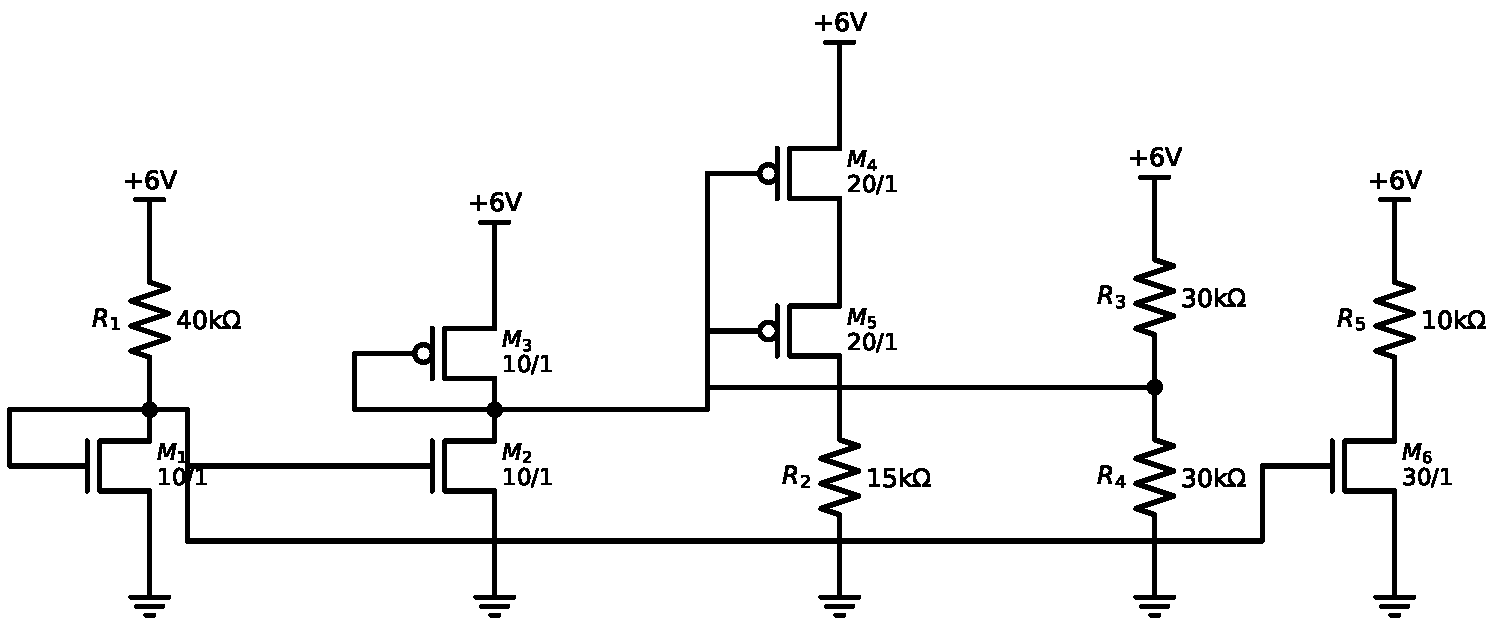
\includegraphics[width=0.9\linewidth,height=6cm,keepaspectratio]{p15_circuit}\end{center}
\solstep{1}{Assumptions}Assume every transistor is active (saturation, tool T1). No current flows into any gate, so gate voltages come from the resistor networks alone.
\solstep{2}{Walk through the circuit}\begin{enumerate}[leftmargin=*,itemsep=3pt]
\item No current flows into a gate ($I_G = 0$), so $V_{G5}$ is set by the divider $R_{3}$--$R_{4}$:\[V_{G5} = 0 + (6 - 0)\frac{30\,\mathrm{k}}{30\,\mathrm{k} + 30\,\mathrm{k}} = 3\,\mathrm{V}\]
\item The reference branch is one series path from $6$ to $0$: $R_{1}$, $M_{1}$. All of them carry the same current $I_D$ (gates draw none), and every diode-connected transistor is active ($V_{DS} = V_{GS} > V_{GS} - V_t$). KVL:\[6 = R_{1}I_D + V_{GS1}\]With $I_D = \frac{2\,\mathrm{m}}{2}(V_{GS1} - 0.7)^2$:\[40V_{GS1}^2 - 55V_{GS1} + 13.6 = 0 \;\Rightarrow\; V_{GS1} = 0.3233\ \text{or}\ 1.052\,\mathrm{V}\]The root $0.323$\,V is below $|V_t| = 0.7$\,V (the transistor would be off), so $V_{GS1} = 1.052$\,V. Hence $I_D = 124\,\mu \mathrm{A}$, and $V_{G1} = 1.05\,\mathrm{V}$.
\item $M_{2}$ has the same gate and source nodes as $M_{1}$, hence the same $V_{GS}$ (current mirror): $I_{D2} = I_{D1} = 124\,\mu \mathrm{A}$.
\item $M_{6}$ has the same gate and source nodes as $M_{1}$, hence the same $V_{GS}$ (current mirror); the currents scale with $W/L$: $I_{D6} = I_{D1}\,\frac{\left(\frac{W}{L}\right)_{6}}{\left(\frac{W}{L}\right)_{1}} = \frac{30/1}{10/1} = 371\,\mu \mathrm{A}$.
\item $I_{D6}$ flows from $6$ through $R_{5}$: $V_{D6} = 6 - R_{5}I_{D6} = 6 - 10\,\mathrm{k}\times371\,\mu \mathrm{A} = 2.29\,\mathrm{V}$.
\item $M_{3}$ is in series with $M_{2}$ (nothing else draws current at $V_{G3}$): $I_{D3} = I_{D2} = 124\,\mu \mathrm{A}$.
\item $M_{4}$ has the same gate and source nodes as $M_{3}$, hence the same $V_{GS}$ (current mirror); the currents scale with $W/L$: $I_{D4} = I_{D3}\,\frac{\left(\frac{W}{L}\right)_{4}}{\left(\frac{W}{L}\right)_{3}} = \frac{20/1}{10/1} = 247\,\mu \mathrm{A}$.
\item $M_{3}$ carries $I_{D3} = 124\,\mu \mathrm{A}$, so $V_{ov3} = \sqrt{2I_{D3}/k_{3}} = 0.4974$\,V and $V_{SG3} = 1.297$\,V: $V_{G3} = 6 - V_{SG3} = 4.7\,\mathrm{V}$ (diode-connected: this is also its drain voltage).
\item $M_{5}$ is in series with $M_{4}$ (nothing else draws current at $V_{D4}$): $I_{D5} = I_{D4} = 247\,\mu \mathrm{A}$.
\item $I_{D5} = 247\,\mu \mathrm{A}$ flows through $R_{2}$ to $0$: $V_{D5} = 0 + R_{2}I_{D5} = 0 + 15\,\mathrm{k}\times247\,\mu \mathrm{A} = 3.71\,\mathrm{V}$.
\item $M_{5}$ carries $I_{D5} = 247\,\mu \mathrm{A}$, so $V_{ov5} = \sqrt{2I_{D5}/k_{5}} = 0.4974$\,V and $V_{SG5} = 0.8 + 0.4974 = 1.297$\,V: $V_{D4} = V_{G5} + V_{SG5} = 4.3\,\mathrm{V}$.
\end{enumerate}

\solstep{3}{Verify the operating modes}\begin{itemize}[leftmargin=*,itemsep=2pt]
\item $M_{1}$ is diode-connected: $V_{DS1} = V_{GS1} > V_{ov1}$, always active \checkmark
\item $M_{3}$ is diode-connected: $V_{SD3} = V_{SG3} > V_{ov3}$, always active \checkmark
\item $V_{DS2} = V_{G3} - 0 = 4.703 - 0 = 4.7\,\mathrm{V}$ $\ge V_{ov2} = 0.352$\,V $\Rightarrow$ $M_{2}$ is active \checkmark
\item $V_{SD4} = 6 - V_{D4} = 6 - 4.297 = 1.7\,\mathrm{V}$ $\ge V_{ov4} = 0.497$\,V $\Rightarrow$ $M_{4}$ is active \checkmark
\item $V_{SD5} = V_{D4} - V_{D5} = 4.297 - 3.711 = 0.586\,\mathrm{V}$ $\ge V_{ov5} = 0.497$\,V $\Rightarrow$ $M_{5}$ is active \checkmark
\item $V_{DS6} = V_{D6} - 0 = 2.289 - 0 = 2.29\,\mathrm{V}$ $\ge V_{ov6} = 0.352$\,V $\Rightarrow$ $M_{6}$ is active \checkmark
\end{itemize}
Unlike the BJT, nothing was neglected here ($I_G = 0$ exactly), so these results are exact for the square-law model: a full nodal solve of the circuit gives the same currents.
\begin{ansbox}
$I_{D1} = 124\,\mu \mathrm{A}$,\quad $I_{D3} = 124\,\mu \mathrm{A}$,\quad $I_{D2} = 124\,\mu \mathrm{A}$,\quad $I_{D4} = 247\,\mu \mathrm{A}$,\quad $I_{D5} = 247\,\mu \mathrm{A}$,\quad $I_{D6} = 371\,\mu \mathrm{A}$\\[2pt] all transistors active.
\end{ansbox}

\newpage
\subsection*{Solution 5B.16 \hfill Hard}
\begin{center}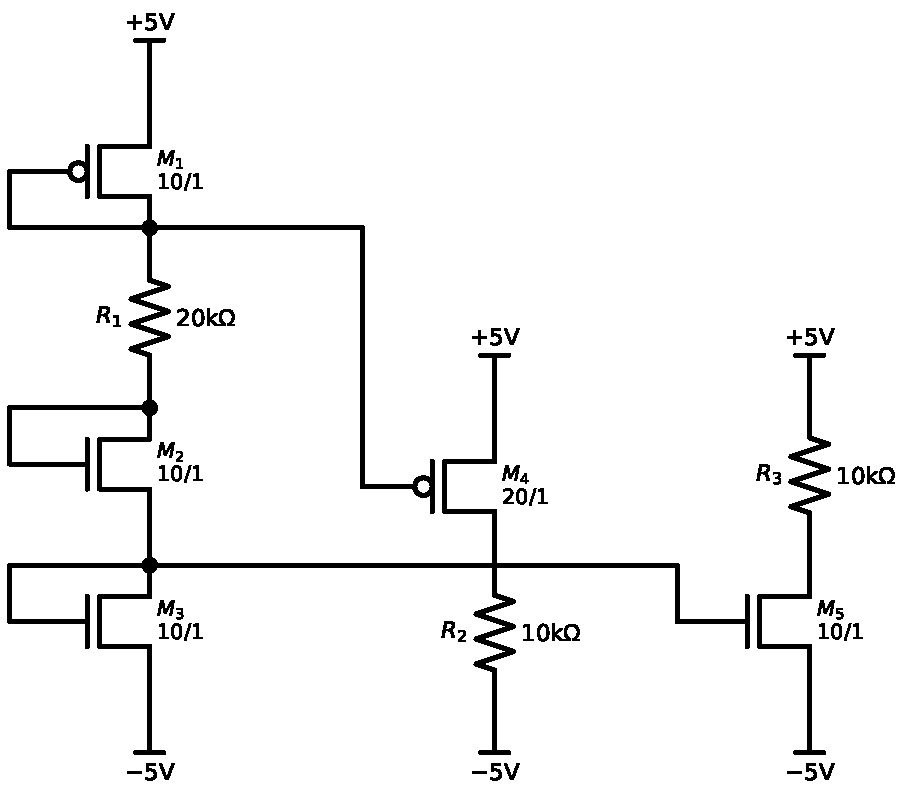
\includegraphics[width=0.9\linewidth,height=6cm,keepaspectratio]{p16_circuit}\end{center}
\solstep{1}{Assumptions}Assume every transistor is active (saturation, tool T1). No current flows into any gate, so gate voltages come from the resistor networks alone.
\solstep{2}{Walk through the circuit}\begin{enumerate}[leftmargin=*,itemsep=3pt]
\item The reference branch is one series path from $5$ to $(-5)$: $M_{1}$, $R_{1}$, $M_{2}$, $M_{3}$. All of them carry the same current $I_D$ (gates draw none), and every diode-connected transistor is active ($V_{DS} = V_{GS} > V_{GS} - V_t$). KVL:\[10 = V_{SG1} + R_{1}I_D + V_{GS2} + V_{GS3}\]Equal currents, $\frac{k_i}{2}V_{ov,i}^2$ the same for all, give $V_{ov2} = V_{ov1}\sqrt{k_{1}/k_{2}} = 0.7071\,V_{ov1}$, $V_{ov3} = V_{ov1}\sqrt{k_{1}/k_{3}} = 0.7071\,V_{ov1}$. With $I_D = \frac{1\,\mathrm{m}}{2}(V_{SG1} - 0.8)^2$ everything is a function of $V_{SG1}$:\[10V_{SG1}^2 - 13.59V_{SG1} - 3.331 = 0 \;\Rightarrow\; V_{SG1} = -0.2121\ \text{or}\ 1.571\,\mathrm{V}\]The root $-0.212$\,V is below $|V_t| = 0.8$\,V (the transistor would be off), so $V_{SG1} = 1.571$\,V. Hence $I_D = 297\,\mu \mathrm{A}$, $V_{GS2} = 1.245$\,V, $V_{GS3} = 1.245$\,V, and $V_{G1} = 3.43\,\mathrm{V}$, $V_{G2} = -2.51\,\mathrm{V}$, $V_{S2} = -3.76\,\mathrm{V}$.
\item $M_{4}$ has the same gate and source nodes as $M_{1}$, hence the same $V_{GS}$ (current mirror); the currents scale with $W/L$: $I_{D4} = I_{D1}\,\frac{\left(\frac{W}{L}\right)_{4}}{\left(\frac{W}{L}\right)_{1}} = \frac{20/1}{10/1} = 594\,\mu \mathrm{A}$.
\item $M_{5}$ has the same gate and source nodes as $M_{3}$, hence the same $V_{GS}$ (current mirror): $I_{D5} = I_{D3} = 297\,\mu \mathrm{A}$.
\item $I_{D4} = 594\,\mu \mathrm{A}$ flows through $R_{2}$ to $(-5)$: $V_{D4} = (-5) + R_{2}I_{D4} = -5 + 10\,\mathrm{k}\times594\,\mu \mathrm{A} = 0.939\,\mathrm{V}$.
\item $I_{D5}$ flows from $5$ through $R_{3}$: $V_{D5} = 5 - R_{3}I_{D5} = 5 - 10\,\mathrm{k}\times297\,\mu \mathrm{A} = 2.03\,\mathrm{V}$.
\end{enumerate}

\solstep{3}{Verify the operating modes}\begin{itemize}[leftmargin=*,itemsep=2pt]
\item $M_{1}$ is diode-connected: $V_{SD1} = V_{SG1} > V_{ov1}$, always active \checkmark
\item $M_{2}$ is diode-connected: $V_{DS2} = V_{GS2} > V_{ov2}$, always active \checkmark
\item $M_{3}$ is diode-connected: $V_{DS3} = V_{GS3} > V_{ov3}$, always active \checkmark
\item $V_{SD4} = 5 - V_{D4} = 5 - 0.9394 = 4.06\,\mathrm{V}$ $\ge V_{ov4} = 0.771$\,V $\Rightarrow$ $M_{4}$ is active \checkmark
\item $V_{DS5} = V_{D5} - (-5) = 2.03 - (-5) = 7.03\,\mathrm{V}$ $\ge V_{ov5} = 0.545$\,V $\Rightarrow$ $M_{5}$ is active \checkmark
\end{itemize}
Unlike the BJT, nothing was neglected here ($I_G = 0$ exactly), so these results are exact for the square-law model: a full nodal solve of the circuit gives the same currents.
\begin{ansbox}
$I_{D1} = 297\,\mu \mathrm{A}$,\quad $I_{D2} = 297\,\mu \mathrm{A}$,\quad $I_{D3} = 297\,\mu \mathrm{A}$,\quad $I_{D4} = 594\,\mu \mathrm{A}$,\quad $I_{D5} = 297\,\mu \mathrm{A}$\\[2pt] all transistors active.
\end{ansbox}

\newpage
\subsection*{Solution 5B.17 \hfill Hard}
\begin{center}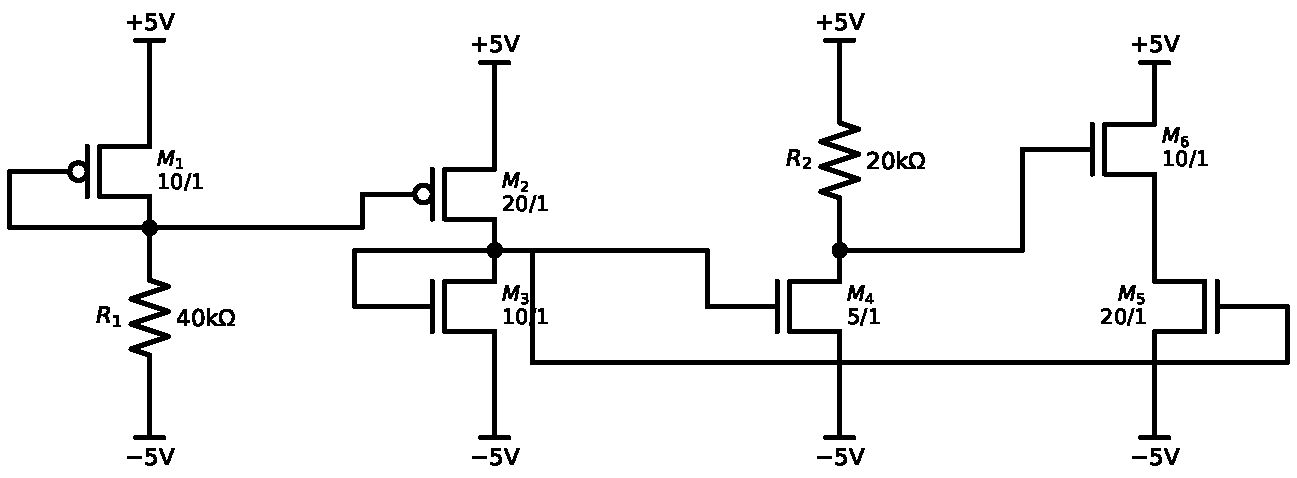
\includegraphics[width=0.9\linewidth,height=6cm,keepaspectratio]{p17_circuit}\end{center}
\solstep{1}{Assumptions}Assume every transistor is active (saturation, tool T1). No current flows into any gate, so gate voltages come from the resistor networks alone.
\solstep{2}{Walk through the circuit}\begin{enumerate}[leftmargin=*,itemsep=3pt]
\item The reference branch is one series path from $5$ to $(-5)$: $M_{1}$, $R_{1}$. All of them carry the same current $I_D$ (gates draw none), and every diode-connected transistor is active ($V_{DS} = V_{GS} > V_{GS} - V_t$). KVL:\[10 = V_{SG1} + R_{1}I_D\]With $I_D = \frac{1\,\mathrm{m}}{2}(V_{SG1} - 0.8)^2$:\[20V_{SG1}^2 - 31V_{SG1} + 2.8 = 0 \;\Rightarrow\; V_{SG1} = 0.09631\ \text{or}\ 1.454\,\mathrm{V}\]The root $0.0963$\,V is below $|V_t| = 0.8$\,V (the transistor would be off), so $V_{SG1} = 1.454$\,V. Hence $I_D = 214\,\mu \mathrm{A}$, and $V_{G1} = 3.55\,\mathrm{V}$.
\item $M_{2}$ has the same gate and source nodes as $M_{1}$, hence the same $V_{GS}$ (current mirror); the currents scale with $W/L$: $I_{D2} = I_{D1}\,\frac{\left(\frac{W}{L}\right)_{2}}{\left(\frac{W}{L}\right)_{1}} = \frac{20/1}{10/1} = 427\,\mu \mathrm{A}$.
\item $M_{3}$ is in series with $M_{2}$ (nothing else draws current at $V_{D2}$): $I_{D3} = I_{D2} = 427\,\mu \mathrm{A}$.
\item $M_{4}$ has the same gate and source nodes as $M_{3}$, hence the same $V_{GS}$ (current mirror); the currents scale with $W/L$: $I_{D4} = I_{D3}\,\frac{\left(\frac{W}{L}\right)_{4}}{\left(\frac{W}{L}\right)_{3}} = \frac{5/1}{10/1} = 214\,\mu \mathrm{A}$.
\item $M_{5}$ has the same gate and source nodes as $M_{3}$, hence the same $V_{GS}$ (current mirror); the currents scale with $W/L$: $I_{D5} = I_{D3}\,\frac{\left(\frac{W}{L}\right)_{5}}{\left(\frac{W}{L}\right)_{3}} = \frac{20/1}{10/1} = 855\,\mu \mathrm{A}$.
\item $M_{3}$ carries $I_{D3} = 427\,\mu \mathrm{A}$, so $V_{ov3} = \sqrt{2I_{D3}/k_{3}} = 0.6537$\,V and $V_{GS3} = 1.354$\,V: $V_{D2} = (-5) + V_{GS3} = -3.65\,\mathrm{V}$ (diode-connected: this is also its drain voltage).
\item $I_{D4}$ flows from $5$ through $R_{2}$: $V_{D4} = 5 - R_{2}I_{D4} = 5 - 20\,\mathrm{k}\times214\,\mu \mathrm{A} = 0.727\,\mathrm{V}$.
\item $M_{6}$ is in series with $M_{5}$ (nothing else draws current at $V_{S6}$): $I_{D6} = I_{D5} = 855\,\mu \mathrm{A}$.
\item $M_{6}$ carries $I_{D6} = 855\,\mu \mathrm{A}$, so $V_{ov6} = \sqrt{2I_{D6}/k_{6}} = 0.9245$\,V and $V_{GS6} = 0.7 + 0.9245 = 1.624$\,V: $V_{S6} = V_{D4} - V_{GS6} = -0.898\,\mathrm{V}$.
\end{enumerate}

\solstep{3}{Verify the operating modes}\begin{itemize}[leftmargin=*,itemsep=2pt]
\item $M_{1}$ is diode-connected: $V_{SD1} = V_{SG1} > V_{ov1}$, always active \checkmark
\item $V_{SD2} = 5 - V_{D2} = 5 - (-3.646) = 8.65\,\mathrm{V}$ $\ge V_{ov2} = 0.654$\,V $\Rightarrow$ $M_{2}$ is active \checkmark
\item $M_{3}$ is diode-connected: $V_{DS3} = V_{GS3} > V_{ov3}$, always active \checkmark
\item $V_{DS4} = V_{D4} - (-5) = 0.7268 - (-5) = 5.73\,\mathrm{V}$ $\ge V_{ov4} = 0.654$\,V $\Rightarrow$ $M_{4}$ is active \checkmark
\item $V_{DS6} = 5 - V_{S6} = 5 - (-0.8976) = 5.9\,\mathrm{V}$ $\ge V_{ov6} = 0.924$\,V $\Rightarrow$ $M_{6}$ is active \checkmark
\item $V_{DS5} = V_{S6} - (-5) = -0.8976 - (-5) = 4.1\,\mathrm{V}$ $\ge V_{ov5} = 0.654$\,V $\Rightarrow$ $M_{5}$ is active \checkmark
\end{itemize}
Unlike the BJT, nothing was neglected here ($I_G = 0$ exactly), so these results are exact for the square-law model: a full nodal solve of the circuit gives the same currents.
\begin{ansbox}
$I_{D1} = 214\,\mu \mathrm{A}$,\quad $I_{D2} = 427\,\mu \mathrm{A}$,\quad $I_{D3} = 427\,\mu \mathrm{A}$,\quad $I_{D4} = 214\,\mu \mathrm{A}$,\quad $I_{D6} = 855\,\mu \mathrm{A}$,\quad $I_{D5} = 855\,\mu \mathrm{A}$\\[2pt] all transistors active.
\end{ansbox}

\newpage
\subsection*{Solution 5B.18 \hfill Hard}
\begin{center}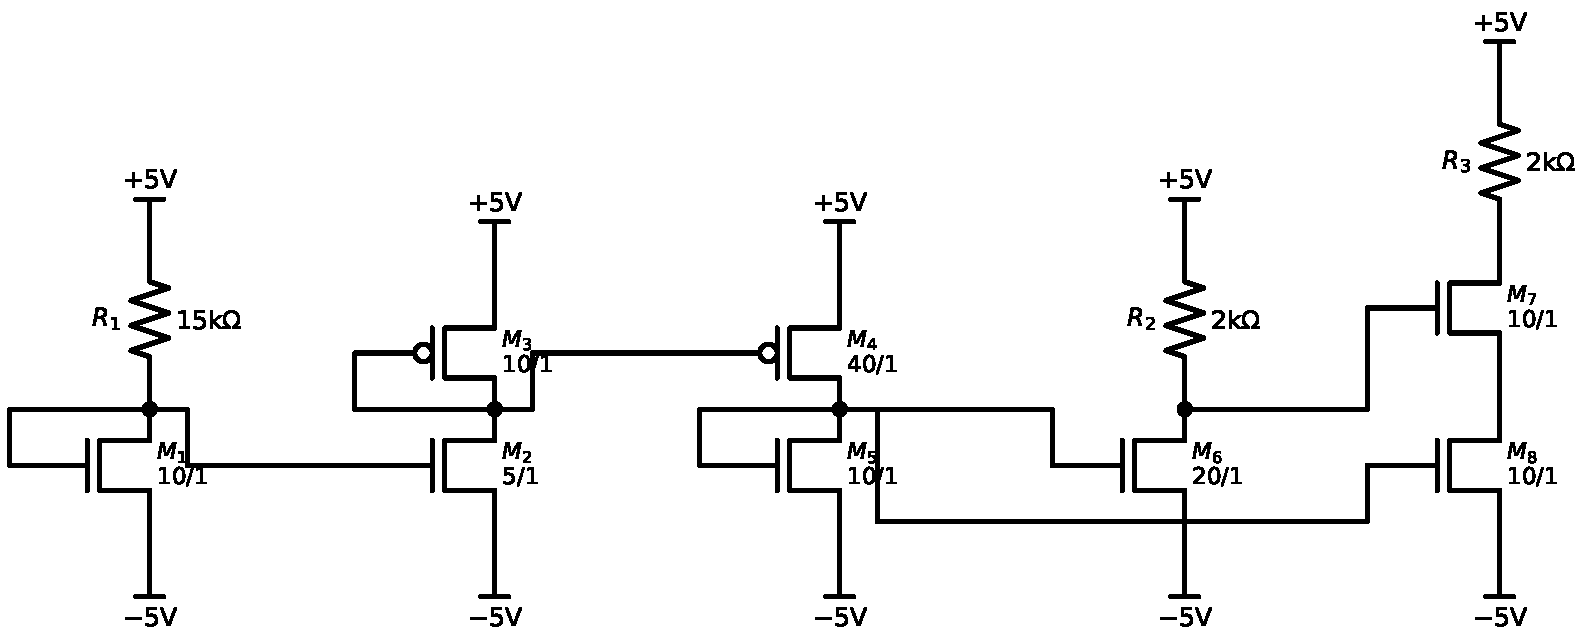
\includegraphics[width=0.9\linewidth,height=6cm,keepaspectratio]{p18_circuit}\end{center}
\solstep{1}{Assumptions}Assume every transistor is active (saturation, tool T1). No current flows into any gate, so gate voltages come from the resistor networks alone.
\solstep{2}{Walk through the circuit}\begin{enumerate}[leftmargin=*,itemsep=3pt]
\item The reference branch is one series path from $5$ to $(-5)$: $R_{1}$, $M_{1}$. All of them carry the same current $I_D$ (gates draw none), and every diode-connected transistor is active ($V_{DS} = V_{GS} > V_{GS} - V_t$). KVL:\[10 = R_{1}I_D + V_{GS1}\]With $I_D = \frac{2\,\mathrm{m}}{2}(V_{GS1} - 0.7)^2$:\[15V_{GS1}^2 - 20V_{GS1} - 2.65 = 0 \;\Rightarrow\; V_{GS1} = -0.1214\ \text{or}\ 1.455\,\mathrm{V}\]The root $-0.121$\,V is below $|V_t| = 0.7$\,V (the transistor would be off), so $V_{GS1} = 1.455$\,V. Hence $I_D = 570\,\mu \mathrm{A}$, and $V_{G1} = -3.55\,\mathrm{V}$.
\item $M_{2}$ has the same gate and source nodes as $M_{1}$, hence the same $V_{GS}$ (current mirror); the currents scale with $W/L$: $I_{D2} = I_{D1}\,\frac{\left(\frac{W}{L}\right)_{2}}{\left(\frac{W}{L}\right)_{1}} = \frac{5/1}{10/1} = 285\,\mu \mathrm{A}$.
\item $M_{3}$ is in series with $M_{2}$ (nothing else draws current at $V_{G3}$): $I_{D3} = I_{D2} = 285\,\mu \mathrm{A}$.
\item $M_{4}$ has the same gate and source nodes as $M_{3}$, hence the same $V_{GS}$ (current mirror); the currents scale with $W/L$: $I_{D4} = I_{D3}\,\frac{\left(\frac{W}{L}\right)_{4}}{\left(\frac{W}{L}\right)_{3}} = \frac{40/1}{10/1} = 1.14\,\mathrm{m}\mathrm{A}$.
\item $M_{3}$ carries $I_{D3} = 285\,\mu \mathrm{A}$, so $V_{ov3} = \sqrt{2I_{D3}/k_{3}} = 0.7548$\,V and $V_{SG3} = 1.555$\,V: $V_{G3} = 5 - V_{SG3} = 3.45\,\mathrm{V}$ (diode-connected: this is also its drain voltage).
\item $M_{5}$ is in series with $M_{4}$ (nothing else draws current at $V_{D4}$): $I_{D5} = I_{D4} = 1.14\,\mathrm{m}\mathrm{A}$.
\item $M_{6}$ has the same gate and source nodes as $M_{5}$, hence the same $V_{GS}$ (current mirror); the currents scale with $W/L$: $I_{D6} = I_{D5}\,\frac{\left(\frac{W}{L}\right)_{6}}{\left(\frac{W}{L}\right)_{5}} = \frac{20/1}{10/1} = 2.28\,\mathrm{m}\mathrm{A}$.
\item $M_{8}$ has the same gate and source nodes as $M_{5}$, hence the same $V_{GS}$ (current mirror): $I_{D8} = I_{D5} = 1.14\,\mathrm{m}\mathrm{A}$.
\item $M_{5}$ carries $I_{D5} = 1.14\,\mathrm{m}\mathrm{A}$, so $V_{ov5} = \sqrt{2I_{D5}/k_{5}} = 1.067$\,V and $V_{GS5} = 1.767$\,V: $V_{D4} = (-5) + V_{GS5} = -3.23\,\mathrm{V}$ (diode-connected: this is also its drain voltage).
\item $I_{D6}$ flows from $5$ through $R_{2}$: $V_{D6} = 5 - R_{2}I_{D6} = 5 - 2\,\mathrm{k}\times2.28\,\mathrm{m}\mathrm{A} = 0.443\,\mathrm{V}$.
\item $M_{7}$ is in series with $M_{8}$ (nothing else draws current at $V_{S7}$): $I_{D7} = I_{D8} = 1.14\,\mathrm{m}\mathrm{A}$.
\item $I_{D7}$ flows from $5$ through $R_{3}$: $V_{D7} = 5 - R_{3}I_{D7} = 5 - 2\,\mathrm{k}\times1.14\,\mathrm{m}\mathrm{A} = 2.72\,\mathrm{V}$.
\item $M_{7}$ carries $I_{D7} = 1.14\,\mathrm{m}\mathrm{A}$, so $V_{ov7} = \sqrt{2I_{D7}/k_{7}} = 1.067$\,V and $V_{GS7} = 0.7 + 1.067 = 1.767$\,V: $V_{S7} = V_{D6} - V_{GS7} = -1.32\,\mathrm{V}$.
\end{enumerate}

\solstep{3}{Verify the operating modes}\begin{itemize}[leftmargin=*,itemsep=2pt]
\item $M_{1}$ is diode-connected: $V_{DS1} = V_{GS1} > V_{ov1}$, always active \checkmark
\item $M_{3}$ is diode-connected: $V_{SD3} = V_{SG3} > V_{ov3}$, always active \checkmark
\item $V_{DS2} = V_{G3} - (-5) = 3.445 - (-5) = 8.45\,\mathrm{V}$ $\ge V_{ov2} = 0.755$\,V $\Rightarrow$ $M_{2}$ is active \checkmark
\item $V_{SD4} = 5 - V_{D4} = 5 - (-3.233) = 8.23\,\mathrm{V}$ $\ge V_{ov4} = 0.755$\,V $\Rightarrow$ $M_{4}$ is active \checkmark
\item $M_{5}$ is diode-connected: $V_{DS5} = V_{GS5} > V_{ov5}$, always active \checkmark
\item $V_{DS6} = V_{D6} - (-5) = 0.4425 - (-5) = 5.44\,\mathrm{V}$ $\ge V_{ov6} = 1.07$\,V $\Rightarrow$ $M_{6}$ is active \checkmark
\item $V_{DS7} = V_{D7} - V_{S7} = 2.721 - (-1.325) = 4.05\,\mathrm{V}$ $\ge V_{ov7} = 1.07$\,V $\Rightarrow$ $M_{7}$ is active \checkmark
\item $V_{DS8} = V_{S7} - (-5) = -1.325 - (-5) = 3.68\,\mathrm{V}$ $\ge V_{ov8} = 1.07$\,V $\Rightarrow$ $M_{8}$ is active \checkmark
\end{itemize}
Unlike the BJT, nothing was neglected here ($I_G = 0$ exactly), so these results are exact for the square-law model: a full nodal solve of the circuit gives the same currents.
\begin{ansbox}
$I_{D1} = 570\,\mu \mathrm{A}$,\quad $I_{D3} = 285\,\mu \mathrm{A}$,\quad $I_{D2} = 285\,\mu \mathrm{A}$,\quad $I_{D4} = 1.14\,\mathrm{m}\mathrm{A}$,\quad $I_{D5} = 1.14\,\mathrm{m}\mathrm{A}$,\quad $I_{D6} = 2.28\,\mathrm{m}\mathrm{A}$,\quad $I_{D7} = 1.14\,\mathrm{m}\mathrm{A}$,\quad $I_{D8} = 1.14\,\mathrm{m}\mathrm{A}$\\[2pt] all transistors active.
\end{ansbox}

\end{document}
